\documentclass[11pt]{article}

\usepackage[left=0.85in,right=0.85in,top=0.8in,bottom=0.8in]{geometry}
\usepackage{amsmath,amssymb,amsthm,mathtools}
\usepackage{enumitem}
\usepackage{tikz}
\usetikzlibrary{arrows.meta,backgrounds,fit,positioning,shapes.geometric}
\usepackage[hidelinks]{hyperref}
\hypersetup{
  pdftitle={Kozma--Nitzan Connection Inequalities for Bernoulli Percolation},
  pdfauthor={ChatGPT 5.6 Sol and Claude Fable 5.1}
}

\newtheorem{theorem}{Theorem}[section]
\newtheorem{lemma}[theorem]{Lemma}
\newtheorem{proposition}[theorem]{Proposition}
\newtheorem{corollary}[theorem]{Corollary}
\theoremstyle{definition}
\newtheorem{conjecture}{Conjecture}
\newtheorem{question}{Question}
\theoremstyle{remark}
\newtheorem{remark}[theorem]{Remark}

\newcommand{\PP}{\mathbb P}
\newcommand{\EE}{\mathbb E}
\newcommand{\one}{\mathbf 1}
\newcommand{\con}{\leftrightarrow}
\newcommand{\ncon}{\nleftrightarrow}
\newcommand{\eC}{\mathcal C}
\DeclareMathOperator{\Cov}{Cov}
\DeclareMathOperator{\vtx}{vtx}
\newcommand{\Marg}{\mathfrak M}

\allowdisplaybreaks

\makeatletter
\def\thm@space@setup{\thm@preskip=0.55\baselineskip \thm@postskip=\thm@preskip}
\makeatother
\AtBeginDocument{%
  \setlength{\abovedisplayskip}{6pt plus 2pt minus 3pt}%
  \setlength{\belowdisplayskip}{6pt plus 2pt minus 3pt}%
  \setlength{\abovedisplayshortskip}{3pt plus 2pt}%
  \setlength{\belowdisplayshortskip}{4pt plus 2pt minus 2pt}%
}

\title{Kozma--Nitzan Connection Inequalities for Bernoulli Percolation}
\author{ChatGPT 5.6 Sol and Claude Fable 5.1}
\date{\small Last Updated: 5 September 2026}

\begin{document}
\maketitle

\begin{center}
\small
The mathematical arguments, exposition, and accompanying Lean formalization were
produced entirely by ChatGPT 5.6 Sol and Claude Fable 5.1, prompted by Ahmed Bou-Rabee.
\par\smallskip
This manuscript accompanies the Lean development in \href{https://github.com/nitromannitol/percolation-after-anthropic}{percolation-after-anthropic}.
\end{center}

\begin{abstract}
Kozma and Nitzan reduced the question whether critical Bernoulli percolation has an
infinite open cluster to connection inequalities on finite weighted graphs. We prove all
five of their conjectures and answer Questions~5, 7, and~9 affirmatively. Question~8 has a
negative answer under the reading that the requested inequality must hold for every
minimizing vertex: a four-vertex graph gives a counterexample. The main argument is a
comparison principle for increasing functions of an open cluster, valid even when the
cluster is conditioned to avoid prescribed vertices. We also prove a version for the
union of the clusters of finitely many starting vertices. These two forms yield the strong
pre-FKG inequality, allow the minimizer in Conjecture~4 to be chosen before conditioning,
remove the two auxiliary inequalities in display~(39) from Conjecture~6, give one
coefficient vector that works simultaneously for every target in Question~5, and prove
Question~9 for every minimizer.
\end{abstract}

\section{Introduction}

In Bernoulli percolation on a finite weighted graph, each edge is open independently with
its prescribed probability. Write $x\con y$ when vertices $x$ and $y$ are joined by an
open path, and write $C_x$ for the open cluster of $x$. Fix two vertices $o$ and $b$, and
think of a nonempty set $A$ as a collection of possible intermediate vertices between
$o$ and $b$. The simplest inequality considered here is
\[
  \PP(o\con b)\geq \PP(o\con A)\min_{x\in A}\PP(x\con b)\,.
\]
The tempting picture is to follow an open path from $o$ until it first meets $A$ and then
continue toward $b$. The difficulty is that the vertex of $A$ selected by the first path is chosen
by the same random configuration that must supply the second path. Thus there are not two
independent connection probabilities to multiply. This dependence created by selecting a
vertex of $A$ through $C_o$ is the probabilistic obstacle in Kozma and Nitzan's reduction
of the critical-percolation problem~\cite{KN}. Their reduction is what makes these finite
graph inequalities worth proving: Conjecture~\ref{c3} below implies that critical Bernoulli
bond percolation on $\mathbb Z^d$ has no infinite open cluster, in every dimension
$d\geq2$.

Kozma and Nitzan separated the problem into five conjectures and four questions. We prove
Conjectures~1, 2, 3, 4, and~6, and we answer Questions~5, 7, and~9 affirmatively. Several
conclusions are stronger than requested. The pre-FKG inequality retains the event
$\{o\con A\}$ on its left side; the minimizing vertex in Conjecture~4 can be selected
before that event is imposed; the hypotheses in display~(39) of Conjecture~6 are
automatic; and the coefficients in Question~5 satisfy a sharper inequality in which $o$
is connected to both $A$ and $b$. Question~8 is the sole exception. Under the reading
that every minimizer must work, a four-vertex graph disproves it as stated.

We begin with a concrete comparison. Let $F$ be an increasing function of a cluster, and
order the vertices of a finite set $T$ by the values $\EE[F(C_x)]$. For each $x\in T$, let
$J_x$ be the event that $x$ is the first vertex in this ordering that belongs to $C_o$.
We prove
\[
  \sum_{x\in T}\PP(J_x)\,\EE[F(C_x)]
  \leq \EE\bigl[F(C_o);\,o\con T\bigr] \,.
\]
Figure~\ref{fig:first-vertex} illustrates this fixed-order selection rule.
\begin{figure}[htbp]
\centering
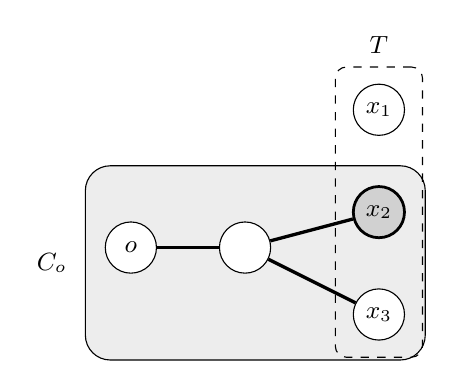
\begin{tikzpicture}[
  vtx/.style={circle,draw,fill=white,inner sep=0pt,minimum size=6.5mm,font=\small},
  sel/.style={vtx,fill=black!18,line width=1pt},
  open/.style={line width=1.2pt}
]
  \node[vtx] (o)  at (0,0)       {$o$};
  \node[vtx] (m)  at (1.45,0)    {};
  \node[vtx] (x1) at (3.15,1.75) {$x_1$};
  \node[sel] (x2) at (3.15,0.45) {$x_2$};
  \node[vtx] (x3) at (3.15,-0.85){$x_3$};
  \draw[open] (o)--(m);
  \draw[open] (m)--(x2);
  \draw[open] (m)--(x3);
  \begin{scope}[on background layer]
    \node[draw,rounded corners=9pt,fill=black!7,fit=(o)(m)(x2)(x3),inner sep=7pt] (co) {};
    \node[draw,dashed,rounded corners=4pt,fit=(x1)(x2)(x3),inner sep=6pt] (tb) {};
  \end{scope}
  \node[anchor=south,font=\small] at (tb.north) [yshift=1pt] {$T$};
  \node[anchor=east,font=\small]  at (co.west)  [xshift=-3pt] {$C_o$};
\end{tikzpicture}
\caption{The vertices of $T$ carry a fixed order $x_1\prec x_2\prec x_3$, chosen before the
configuration is sampled. Here $T\cap C_o=\{x_2,x_3\}$, so $J_{x_2}$ occurs and $x_2$ is
shaded. Nothing is traversed: the vertex is selected by this fixed order, not by order of
arrival along a path.}
\label{fig:first-vertex}
\end{figure}
Although $C_o=C_x$ on $J_x$, conditioning on $J_x$ changes the law of the cluster; the
inequality controls this dependence. We first prove a form conditioned on the cluster
avoiding a fixed set $Y$. The increasing function $\Phi_a$ introduced in
Section~\ref{sec:proj} then converts conditional expectations into differences of
unconditional expectations. The
result is the following useful principle: if $a\in A$ minimizes $\EE[F(C_x)]$ over
$x\in A$, then
\[
  \EE\bigl[F(C_a);\,o\con A\bigr]
  \leq \EE\bigl[F(C_o);\,o\con A\bigr] \,.
\]
Taking $F$ to indicate connection to $b$ proves Conjectures~1--3 and Question~7. General
increasing functions give Conjecture~4, while finite-dimensional separation produces the
single coefficient vector required in Question~5.

Conjecture~6 and Question~9 require the same comparison with several starting vertices.
We replace $C_o$ by $C_R=\bigcup_{x\in R}C_x$ for a nonempty set $R$. When $R$ consists
of the two endpoints of an edge, $C_R$ does not depend on whether that edge is open; forcing
the edge open therefore gives Conjecture~6. For Question~9, we expose the edges incident
to $o$. Conditional on their states, $C_o$ is the union of the clusters starting from $o$
and its open neighbors, so the comparison for $C_R$ applies.

The exposition does not assume familiarity with the Kozma--Nitzan paper. Section~\ref{sec:model}
defines the model and states all nine items in full. Section~\ref{sec:inputs} states the
correlation inequalities used as inputs. Sections~\ref{sec:gen}--\ref{sec:q5} prove the
comparison for one starting vertex and its first applications. Sections~\ref{sec:c6}
and~\ref{sec:q9} treat several starting vertices. Section~\ref{sec:q8} gives the
counterexample to Question~8. Section~\ref{sec:lean} describes the accompanying Lean
verification.

\section{Model and Statements}\label{sec:model}

We now state the model and the nine Kozma--Nitzan problems in the present notation, making
the paper independent of the notation of~\cite{KN} and making the tie interpretation of
Question~\ref{q8} explicit.

Let $V$ be a finite set. Each two-element subset $e\subseteq V$ is an edge. Fix an
edge-opening probability $p_e\in[0,1]$ and declare the edges open independently, with $e$
open with probability $p_e$. An edge with $p_e=0$ may be regarded as absent. We identify a
configuration $\omega$ with its set of open edges and write $\Omega$ for the finite set of
all configurations. Write $\PP$ and $\EE$ for the resulting probability and expectation.
For an event $E$, set $\EE[X;E]=\EE[X\one_E]$. Inside $\PP(\cdot)$, and after the
semicolon in $\EE[\cdot\,;\cdot]$, a comma denotes intersection of events. We use the
conventions that an empty intersection of events is the whole space, an empty union is
empty, an empty sum is zero and an empty product is one.

For vertices $x$ and $y$, write $x\con y$ when there is a path of open edges from $x$ to
$y$, and $x\ncon y$ otherwise. Connection is reflexive, so $x\con x$ always. Write
$C_x=\{y\in V:x\con y\}$ for the open cluster of $x$, and $\eC_x$ for the set of open edges
with at least one endpoint in $C_x$. For an edge set $K$, let $\vtx K$ be the set of
vertices incident to an edge of $K$, so that $C_x=\{x\}\cup\vtx\eC_x$.

For vertex sets $R,B\subseteq V$, put $C_R=\bigcup_{r\in R}C_r$ and write
$\{R\con B\}=\{C_R\cap B\neq\varnothing\}$; write $\{R\ncon B\}$ for its complement. For
$R=\{x\}$ we abbreviate these events to $\{x\con B\}$ and $\{x\ncon B\}$. Write $\eC_R$
for the set of open edges with at least one endpoint in $C_R$. The indicator of an
event is written $\one_A$ when the event has been given the name $A$, and
$\one\{\,\cdot\,\}$ when it is written out. A function $F$ from subsets of $V$ to the real
numbers is increasing when $K\subseteq L$ implies $F(K)\leq F(L)$. Every set in this note is
finite because $V$ is finite, and $A$ is always a nonempty subset of $V$. Throughout the
paper $V$ is the vertex set of a finite weighted graph and $\PP$ and $\EE$ are its
probability and expectation, and every statement below is made in this setting.

Kozma and Nitzan write $\PP(0\con b)$ where we write $\PP(o\con b)$. They call a function
$f$ of a vertex and a configuration a monotone cluster property when two conditions hold:
$f(v,\omega)$ depends only on the open cluster of $v$ and is increasing under inclusion of
that cluster, and an open edge $\{v,w\}$ implies $f(v,\omega)=f(w,\omega)$. Their five conjectures and four questions are the
following; there is no Conjecture 5 and no Question 6.

\begin{conjecture}[Kozma and Nitzan, display (1)]\label{c1}
Let $o$ and $b$ be vertices and let $A$ be a nonempty set of vertices. Then
\[
 \PP(o\con b)\geq \PP(o\con A)\,\min_{x\in A}\PP(x\con b)\,.
\]
\end{conjecture}

For each $x\in A$, Harris's inequality gives
$\PP(o\con A,x\con b)\geq\PP(o\con A)\PP(x\con b)$. Thus Conjecture~2 is formally stronger
than Conjecture~1.

\begin{conjecture}[Kozma and Nitzan, display (2)]\label{c2}
Let $o$ and $b$ be vertices and let $A$ be a nonempty set of vertices. Then
\[
 \PP(o\con b)\geq \min_{x\in A}\PP(o\con A,\ x\con b)\,.
\]
\end{conjecture}

Kozma and Nitzan call Conjecture~\ref{c1} the post-FKG conjecture and Conjecture~\ref{c2}
the pre-FKG conjecture. They record the formally stronger form
\begin{equation}\label{eq:pre}
 \PP(o\con b,\ o\con A)\geq \min_{x\in A}\PP(o\con A,\ x\con b)\,,
\end{equation}
their display (3).

The reduction to the infinite-volume problem needs the following uniform near-one form.

\begin{conjecture}[Kozma and Nitzan, page 15]\label{c3}
For every $\varepsilon>0$ there exists $\delta>0$ such that, for every finite weighted graph
with vertex set $V$, every nonempty $A\subseteq V$, and all $o,b\in V$, the following
implication holds: if $\PP(o\con A)>1-\delta$ and $\PP(x\con b)>1-\delta$ for every
$x\in A$, then $\PP(o\con b)>1-\varepsilon$.
\end{conjecture}

The next conjecture replaces the connection indicator by an arbitrary monotone cluster
property.

\begin{conjecture}[Kozma and Nitzan, page 32]\label{c4}
Let $f$ be a monotone cluster property, let $A$ be a nonempty set of vertices and let $o$
be a vertex. Then
\[
 \EE\bigl[f(o,\cdot);\,o\con A\bigr]\geq \min_{x\in A}\EE\bigl[f(x,\cdot);\,o\con A\bigr]\,.
\]
\end{conjecture}

For an edge $e$, write $\PP^e$ and $\EE^e$ for probability and expectation under the law
obtained by setting $p_e=1$ and leaving all other edge probabilities unchanged. Kozma and
Nitzan write $G\downarrow e$ for the corresponding graph; for connection events, this is
equivalent to contracting $e$.

\setcounter{conjecture}{5}
\begin{conjecture}[Kozma and Nitzan, displays (39) and (40)]\label{c6}
Let $A$ be a nonempty set of vertices, let $b$ be a vertex, let $a\in A$ satisfy
$\PP(a\con b)\leq\PP(x\con b)$ for every $x\in A$, and let $e=\{v,w\}$ be an edge. Assume
\begin{equation}\label{eq:39}
 \PP(x\con b)\geq \PP(x\con A)\,\PP(a\con b)\qquad\text{for } x=v \text{ and } x=w\,.
\end{equation}
Then
\begin{equation}\label{eq:40}
 \PP^e(v\con b)\geq \PP^e(v\con A)\,\PP^e(a\con b)\,.
\end{equation}
\end{conjecture}

\setcounter{question}{4}
\begin{question}[Kozma and Nitzan, display (38)]\label{q5}
Let $A$ be a nonempty set of vertices and let $o$ be a vertex. Do there exist coefficients
$(c_x)_{x\in A}$, depending on $A$ and on $o$ and on the edge probabilities but not on $b$, such
that every $c_x$ is nonnegative and $\sum_{x\in A}c_x=1$ and, for every $b\in V$,
\[
 \PP(o\con b)\geq \sum_{x\in A}c_x\,\PP(o\con A,\ x\con b)?
\]
\end{question}

The last three questions all ask whether a specified vertex $a\in A$ satisfies the
inequality of the paper's display (41),
\begin{equation}\label{eq:41}
 \PP(o\con b,\ o\con A)\geq \PP(o\con A,\ a\con b)\,.
\end{equation}

\setcounter{question}{6}
\begin{question}[Kozma and Nitzan, page 36]\label{q7}
Let $A$ be a nonempty set of vertices, let $o$ and $b$ be vertices, and let $a\in A$
satisfy $\PP(a\con b)\leq\PP(x\con b)$ for every $x\in A$. Must
\[
 \PP(o\con b,\ o\con A)\geq \PP(o\con A,\ a\con b)
\]
hold?
\end{question}

Question~8 instead selects the vertex by minimizing under the complementary event
$\{o\ncon A\}$. The printed question says to let $a$ be a minimizing point and does not
specify what happens when the minimum is attained more than once. We state the reading
under which the inequality is required for every minimizing vertex.

\begin{question}[universal-minimizer reading of Kozma and Nitzan, page 36]\label{q8}
Let $A$ be a nonempty set of vertices and let $o,b\in V$. Must the following inequality
hold for every $a\in A$ satisfying
$\PP(a\con b,\ o\ncon A)\leq\PP(x\con b,\ o\ncon A)$ for every $x\in A$?
\[
 \PP(o\con b,\ o\con A)\geq \PP(o\con A,\ a\con b)
\]
\end{question}

For a vertex $o$, let $\PP_\star$ and $\EE_\star$ be the probability and the expectation in
the percolation measure in which every edge incident to $o$ is closed and all other edge
probabilities are unchanged.

\begin{question}[Kozma and Nitzan, page 36]\label{q9}
Let $A$ be a nonempty set of vertices, let $o$ and $b$ be vertices, and let $a\in A$
satisfy $\PP_\star(a\con b)\leq\PP_\star(x\con b)$ for every $x\in A$. With both
probabilities evaluated in the
original measure, must
\[
 \PP(o\con b,\ o\con A)\geq \PP(o\con A,\ a\con b)
\]
hold?
\end{question}

The quantity minimized in Question~\ref{q8} is the probability that $x$ is connected to
$b$ and $o$ is not connected to $A$. It differs from the quantity on the right side of
\eqref{eq:41}, which is treated by \eqref{eq:pre}.

Section~\ref{sec:inputs} states the correlation inequalities that control the dependence
between the cluster reaching $A$ and the choice of a vertex in $A$.

\section{Correlation Inputs}\label{sec:inputs}

Four inputs are used, and this section states each one in the form in which
Sections~\ref{sec:gen} and~\ref{sec:c6} apply it. The first two are correlation
inequalities of van den Berg, H\"aggstr\"om and Kahn: one for two increasing functions of a
single cluster conditioned to avoid a set, and one for two clusters conditioned to be
disconnected from each other. The third is the conditional covariance inequality
of~\cite{Dev}, the source of the machine-checked proof of Conjecture~\ref{c3}. The fourth
consists of two identities that express the domain Markov property, together with a stopped
covariance estimate.

The first input is the conditional positive-association inequality of van den Berg,
H\"aggstr\"om and Kahn~\cite{BHK}.

\begin{theorem}[van den Berg, H\"aggstr\"om and Kahn]\label{thm:bhk}
Let $s$ be a vertex, let $X_1$ and $X_2$ be sets of vertices not containing $s$ and let
$g_1$ and $g_2$ be nonnegative increasing functions of edge sets. Then
\[
 \EE\bigl[g_1(\eC_s);\,s\ncon X_1\bigr]\,\EE\bigl[g_2(\eC_s);\,s\ncon X_2\bigr]
\leq \EE\bigl[g_1(\eC_s)g_2(\eC_s);\,s\ncon (X_1\cap X_2)\bigr]\,
       \PP\bigl(s\ncon (X_1\cup X_2)\bigr)\,.
\]
\end{theorem}

A companion inequality of the same authors governs two clusters at once.

\begin{theorem}[van den Berg, H\"aggstr\"om and Kahn]\label{thm:bhk2}
Let $S_1$ and $S_2$ be sets of vertices, and let $g_3$ and $g_4$ be real functions of two
edge sets, both increasing in the first argument and decreasing in the second. Let
$D=\{S_1\ncon S_2\}$ and, for $i=3,4$, set
$G_i(\omega)=g_i(\eC_{S_1}(\omega),\eC_{S_2}(\omega))$. Then
\[
 \EE[G_3;D]\,\EE[G_4;D]\leq \PP(D)\,\EE[G_3G_4;D]\,.
\]
\end{theorem}

Exchanging $S_1$ and $S_2$ shows that Theorem~\ref{thm:bhk2} also holds when $g_3$ and
$g_4$ are both decreasing in the first argument and increasing in the second. Replacing
$g_4$ by $-g_4$ reverses the inequality:
\begin{equation}\label{eq:bhkneg}
 \PP(S_1\ncon S_2)\,\EE\bigl[g_3g_4;\,S_1\ncon S_2\bigr]\leq
 \EE\bigl[g_3;\,S_1\ncon S_2\bigr]\,\EE\bigl[g_4;\,S_1\ncon S_2\bigr]\,,
\end{equation}
when one of the two functions is increasing in the first argument and decreasing in the
second while the other is decreasing in the first and increasing in the second.

Taking $X_1=X_2$ in Theorem~\ref{thm:bhk} gives the conditional positive association of two
increasing functions of a single cluster,
\begin{equation}\label{eq:bhk1}
 \EE\bigl[g_1(\eC_s);\,s\ncon X\bigr]\,\EE\bigl[g_2(\eC_s);\,s\ncon X\bigr]
\leq \PP(s\ncon X)\,\EE\bigl[g_1(\eC_s)g_2(\eC_s);\,s\ncon X\bigr]\,.
\end{equation}
Because the edge-cluster state space is finite, we may add constants that make $g_1$ and
$g_2$ nonnegative. Adding a constant to either function changes the two sides of
\eqref{eq:bhk1} by the same quantity. Thus \eqref{eq:bhk1} holds for arbitrary real-valued
increasing $g_1,g_2$. Taking $g_1=g_2=1$ in Theorem~\ref{thm:bhk} gives Harris's inequality
for the two avoidance events $\{s\ncon X_1\}$ and $\{s\ncon X_2\}$. We also use Harris's
inequality~\cite{H} for increasing events and the Ahlswede--Daykin four-functions
theorem~\cite{AD}.

The second input is a conditional covariance inequality with finitely many correction
terms. Theorem~\ref{thm:csh} is imported from the machine-checked proof~\cite{Dev}. We
state its precise probabilistic form so that no normalization or conditioning convention
is left implicit; Section~\ref{sec:lean} gives the corresponding Lean declaration.

Fix a vertex $s$, a set $Y$ of vertices with $s\notin Y$, a list $z_1,\dots,z_\ell$ of
distinct vertices and two further distinct vertices $o$ and $v$, all the named vertices
lying outside $Y$ and being pairwise distinct. Write $\nu$ for the conditional law
$\PP(\,\cdot\mid s\ncon Y)$ and put
\begin{equation}\label{eq:constants}
 \pi_j(u)=\PP\bigl(u\in C_{z_j}\bigm|z_j\ncon B_j\bigr),\qquad
 \tau=\PP\bigl(o\in C_v\bigm|v\ncon B_{\ell+1}\bigr)\,,
\end{equation}
where $B_1=\{s\}\cup Y$ and $B_{j+1}=B_j\cup\{z_j\}$ for $1\leq j\leq\ell$. For a real
function $q$ on $V$ put $q^0=q$ and
\begin{equation}\label{eq:levels}
 q^j(u)=q^{j-1}(u)-\pi_j(u)\,q^{j-1}(z_j)\quad\text{for } 1\leq j\leq\ell,\qquad
 \Marg[q]=q^\ell(o)-\tau\,q^\ell(v)\,.
\end{equation}
The $j$th step subtracts from the value at $u$ the value at $z_j$, multiplied by the
conditional connection probability $\pi_j(u)$. All constants are computed under $\PP$,
not under $\nu$.

\begin{theorem}\label{thm:csh}
Let $V$ be a finite vertex set with every edge probability strictly between zero and one, let
$Y\subseteq V$, let $s$ be a vertex outside $Y$, let $z_1,\dots,z_\ell$ be distinct
vertices outside $Y\cup\{s\}$, let $o$ and $v$ be two further distinct vertices outside
$Y\cup\{s,z_1,\dots,z_\ell\}$, and let $g$ be an increasing function of edge sets.
Put $B_1=\{s\}\cup Y$ and $B_{j+1}=B_j\cup\{z_j\}$. Define
\[
 \pi_j(u)=\PP\bigl(u\in C_{z_j}\mid z_j\ncon B_j\bigr),\qquad
 \tau=\PP\bigl(o\in C_v\mid v\ncon B_{\ell+1}\bigr),
\]
and let $\nu=\PP(\,\cdot\mid s\ncon Y)$. Set
$\kappa(u)=\Cov_\nu(g(\eC_s),\one\{u\in C_s\})$, and recursively define
$\kappa^0=\kappa$ and
\[
 \kappa^j(u)=\kappa^{j-1}(u)-\pi_j(u)\kappa^{j-1}(z_j)
 \qquad (1\leq j\leq\ell).
\]
Then
\[
 \kappa^\ell(o)-\tau\kappa^\ell(v)\geq0.
\]
\end{theorem}

For $\ell=0$ the conclusion reads
\[
 \Cov_\nu\bigl(g(\eC_s),\one\{o\in C_s\}\bigr)\geq
 \PP\bigl(o\in C_v\bigm|v\ncon\{s\}\cup Y\bigr)\,\Cov_\nu\bigl(g(\eC_s),\one\{v\in C_s\}\bigr)\,,
\]
If moreover $Y=\varnothing$ and
$g(K)=\one\{v\in\{s\}\cup\vtx K\}$, then the displayed inequality is equivalent to Harris's
inequality for the increasing events $\{s\con v\}$ and
$\{s\con o\}\cup\{v\con o\}$.

For the remaining two inputs, fix a vertex $s$, a set $Y$ not containing $s$, and an
increasing function $g$ of edge sets. We first use a cluster-exploration consequence of
the domain Markov property, in the form of BHK's cluster-conditioning lemma
\cite[Lemma~2.4]{BHK}. Expose the edge cluster $\eC_Y$ and condition on its value. On the event $D=\{s\ncon Y\}$, the vertex set
$C_Y=Y\cup\vtx\eC_Y$ is disjoint from $C_s$, every edge with exactly one endpoint in
$C_Y$ is closed, and the edges with both endpoints outside $C_Y$ retain their original
probabilities and are independent of the edges
meeting $C_Y$.

For a vertex set $K$, write $\bar g(K)=\EE_{V\setminus K}[g(\eC_s)]$ for the expectation of
$g(\eC_s)$ in the measure in which every edge meeting $K$ is closed and every remaining edge
keeps its original probability. The exposed cluster $C_Y$ is random, so $\bar g(C_Y)$ is a
random variable, and
\begin{equation}\label{eq:resid}
 \Theta=\one_D\bigl(g(\eC_s)-\bar g(C_Y)\bigr)
\end{equation}
has $\EE[\Theta\mid\eC_Y]=0$. For every vertex set $K$, let
$\Psi(K)$ be minus the expectation of $\Theta$ under the product measure in which every edge meeting
$K$ is closed. Then $\Psi(\varnothing)=0$, the function $\Psi$ is nonnegative and
increasing, and for every vertex $z$ and every set $B$ containing $\{s\}\cup Y$ but not $z$,
\begin{equation}\label{eq:markov1}
 \EE\bigl[\Theta;\,z\ncon B\bigr]=-\,\EE\bigl[\Psi(C_z);\,z\ncon B\bigr]\,.
\end{equation}
The conditional-mean identity and \eqref{eq:markov1} express the domain Markov property:
given $\eC_B$, the edges with both endpoints outside $C_B$ retain their original
probabilities and are independent of the exposed cluster.

We also need the following stopped conditional covariance estimate. It follows from
Gladkov's decision-tree Harris--Kleitman inequality~\cite[Theorem~3.2]{Gladkov24} together
with the BHK cluster inequalities; its machine-checked formulation is identified in
Section~\ref{sec:lean}. For a set
$W$ of vertices use the subscript $W$ on $\PP$ and on $\EE$ and on $\Cov$ for the
probability, the expectation and the covariance in the percolation measure in which every edge with an endpoint outside
$W$ is closed and every edge with both endpoints in $W$ keeps its probability. For a set $X$ of
vertices containing $s$ and a vertex $v\notin X$, put
\begin{equation}\label{eq:etadef}
 \eta_v(W)=\Cov_W\bigl(g(\eC_s),\one\{v\con X\}\bigr)\ \text{ for } v\in W,
 \qquad \eta_v(W)=0\ \text{ for } v\notin W\,.
\end{equation}
Then for every $W$ and every $Q\subseteq W$,
\begin{equation}\label{eq:stopped}
 \EE_W\bigl[\one\{s\ncon Q\}\,\eta_v(W\setminus C_Q)\bigr]\,\PP_W(v\ncon X)
\leq \PP_W\bigl(v\ncon X\cup Q\bigr)\,\eta_v(W)\,,
\end{equation}
and the left side of \eqref{eq:stopped} decreases as $Q$ grows.

Theorem~\ref{thm:gen} turns these correlation inputs into a comparison for the vertex of
$T$ selected by the cluster of $o$. The conditioning on avoiding $Y$ is essential: in
Section~\ref{sec:proj} we take $Y=\{a\}$, where $a$ is the proposed minimizer.

\section{A Conditional Comparison}\label{sec:gen}

Our first main estimate controls the bias caused by selecting a vertex of $T$ through the
cluster of $o$. We prove it while requiring that cluster to avoid a fixed set $Y$.

Throughout this section $V$ is a finite vertex set with edge probabilities in $[0,1]$, the set
$Y$ is a subset of $V$, and $F$ is an increasing function of subsets of $V$. For a vertex
$x$ with $\PP(x\ncon Y)>0$ put
\begin{equation}\label{eq:condmean}
 m_x=\frac{\EE\bigl[F(C_x);\,x\ncon Y\bigr]}{\PP(x\ncon Y)}\,,
\end{equation}
the conditional expectation of $F(C_x)$ given $x\ncon Y$. Also fix a set $T\subseteq V\setminus Y$
with $\PP(x\ncon Y)>0$ for every $x\in T$, and an injective real function $r$ on $T$ with
$m_x\leq m_y$ whenever $r(x)<r(y)$. Such an $r$ exists: order $T$ by the values $m_x$ and
break ties arbitrarily. For $x\in T$ and a vertex $o$ write
\begin{equation}\label{eq:pattern}
 J_x=\{o\ncon Y\}\cap\{o\con x\}\cap\bigcap_{y\in T,\ r(y)<r(x)}\{o\ncon y\}
\end{equation}
for the event that $o$ is not connected to $Y$ and $x$ is the vertex of smallest value of
$r$ in $T\cap C_o$. The events $J_x$ are disjoint and their union is
$\{o\ncon Y\}\cap\{o\con T\}$. Put
\begin{equation}\label{eq:surplus}
 \Lambda_o(T)=\EE\bigl[F(C_o);\,o\ncon Y,\ o\con T\bigr]-\sum_{x\in T}\PP(J_x)\,m_x\,.
\end{equation}

On $J_x$ the vertex $x$ has the smallest value of $r$ among the vertices of $T$ in $C_o$,
hence the smallest value of $m$, and on $J_x$ the clusters $C_o$ and $C_x$ coincide.
Consequently \eqref{eq:surplus} admits the expression
\begin{equation}\label{eq:minform}
 \Lambda_o(T)=\EE\Bigl[\one\{o\ncon Y,\,o\con T\}\Bigl(F(C_o)-\min_{x\in T\cap C_o}
 m_x\Bigr)\Bigr]\,,
\end{equation}
which does not refer to $r$. If $T\cap C_o=\varnothing$, then the indicator in
\eqref{eq:minform} is zero, so assigning the value zero to the empty minimum does not
affect the expectation.

Two cases are immediate. If $o\in Y$, then the event $\{o\ncon Y\}$ is
empty and $\Lambda_o(T)=0$. If $o\in T$, then $o\in T\cap C_o$ on $\{o\ncon Y\}$, so the
minimum in \eqref{eq:minform} is at most $m_o$, whence
$\Lambda_o(T)\geq\EE[F(C_o)-m_o;\,o\ncon Y]=0$ by \eqref{eq:condmean}.

\begin{theorem}\label{thm:gen}
Let $V$ be the vertex set of a finite weighted graph, let $Y\subseteq V$, let
$F:2^V\to\mathbb R$ be
increasing, and let $T\subseteq V\setminus Y$ satisfy $\PP(x\ncon Y)>0$ for every $x\in T$.
Set
\[
 m_x=\frac{\EE[F(C_x);x\ncon Y]}{\PP(x\ncon Y)}
\]
and choose an injective $r:T\to\mathbb R$ such that $m_x\leq m_y$ whenever
$r(x)<r(y)$. For $o\in V$ and $x\in T$, set
\[
 J_x=\{o\ncon Y,o\con x\}\cap
      \bigcap_{\substack{y\in T\\r(y)<r(x)}}\{o\ncon y\}.
\]
Then
\[
 \sum_{x\in T}\PP(J_x)\,m_x\leq \EE\bigl[F(C_o);\,o\ncon Y,\ o\con T\bigr]\,.
\]
\end{theorem}

For $Y=\varnothing$ this is the inequality quoted in the introduction. No sign hypothesis
on $F$ is needed. The proof removes from $T$ the vertex with the largest value of $m$.
The following consequence of Theorem~\ref{thm:csh} controls the possible negative term
introduced by this removal.

\begin{proposition}\label{prop:s5}
Let $V$ be the vertex set of a finite weighted graph, let $Y\subseteq V$, let
$F:2^V\to\mathbb R$ be increasing, and let $T\subseteq V\setminus Y$ satisfy
$\PP(x\ncon Y)>0$ for every $x\in T$. Define
\[
 m_x=\frac{\EE[F(C_x);x\ncon Y]}{\PP(x\ncon Y)}
\]
and let $r:T\to\mathbb R$ be injective with $m_x\leq m_y$ whenever $r(x)<r(y)$. For
$u\in V$, define
\[
 \Lambda_u(T)=\EE[F(C_u);u\ncon Y,u\con T]
 -\sum_{x\in T}\PP\left(
   \{u\ncon Y,u\con x\}\cap
   \bigcap_{\substack{y\in T\\r(y)<r(x)}}\{u\ncon y\}\right)m_x .
\]
If $v\in V\setminus(Y\cup T)$, then, for every $o\in V$,
\[
 \PP\bigl(v\ncon Y\cup T,\ o\con v\bigr)\,\Lambda_v(T)
\leq \PP\bigl(v\ncon Y\cup T\bigr)\,\Lambda_o(T)\,.
\]
\end{proposition}

\begin{proof}
We proceed in three steps: an induction on the cardinality of $T$, its specialization to an
empty list of auxiliary vertices, and the passage to weights in $[0,1]$.

Assume first that every edge probability lies strictly between zero and one, that $o$ lies
outside $Y\cup T$ and that $o\neq v$. Let $z_1,\dots,z_\ell$ be distinct vertices outside
$Y\cup T\cup\{o,v\}$. Put $B_1=Y\cup T$ and $B_{j+1}=B_j\cup\{z_j\}$, and let $\Marg$ be the functional
\eqref{eq:levels} built from the constants
$\pi_j(u)=\PP(u\in C_{z_j}\mid z_j\ncon B_j)$ and
$\tau=\PP(o\in C_v\mid v\ncon B_{\ell+1})$. We start by
showing, by induction on the cardinality of $T$ and simultaneously for every such list and
every pair of vertices $o$ and $v$, that
\begin{equation}\label{eq:s5d}
 \Marg\bigl[\,u\mapsto\Lambda_u(T)\,\bigr]\geq 0\,.
\end{equation}

In the base case $T=\varnothing$ each $\Lambda_u(\varnothing)$ vanishes. For the inductive
step, let $T$ be nonempty, let $k\in T$ have the largest value of $r$, and put
$T_0=T\setminus\{k\}$. For a vertex $u$ put
\[
 p(u)=\PP\bigl(k\ncon Y\cup T_0,\ u\con k\bigr),\qquad
 \mu(u)=\EE\bigl[F(C_k);\,k\ncon Y\cup T_0,\ u\con k\bigr]\,.
\]
Connection is reflexive, so the event $\{k\con k\}$ is the whole space, and the values at
$u=k$ are $p(k)=\PP(k\ncon Y\cup T_0)$ and
$\mu(k)=\EE[F(C_k);\,k\ncon Y\cup T_0]$.

Since $k$ has the largest value of $r$, adding $k$ to $T_0$ leaves the events $J_x$ for
$x\in T_0$ unchanged and creates the single new event $\{k\ncon Y\cup T_0,\ u\con k\}$: on
$\{u\con k\}$ the clusters of $u$ and $k$ coincide. On that event $F(C_u)=F(C_k)$, so
\begin{equation}\label{eq:peel}
 \Lambda_u(T)=\Lambda_u(T_0)+\mu(u)-p(u)\,m_k\,.
\end{equation}

Write $\chi(u)$ for $p(k)\,\mu(u)-\mu(k)\,p(u)$. If $\kappa$ denotes the conditional
covariance of Theorem~\ref{thm:csh} for the vertex $k$, the set $Y\cup T_0$ and the
increasing function $\eC\mapsto F(\{k\}\cup\vtx\eC)$, then $\chi(u)=p(k)^2\kappa(u)$.
Since $p(k)>0$ and $\Marg$ is linear, the two statements $\Marg[\chi]\geq0$ and
$\Marg[\kappa]\geq0$ are equivalent. Put $\gamma_k=m_k\,p(k)-\mu(k)$. Expanding
both sides gives
\begin{equation}\label{eq:covid}
 p(k)\bigl(\mu(u)-p(u)\,m_k\bigr)=\chi(u)-\gamma_k\,p(u)\,.
\end{equation}

Apply Theorem~\ref{thm:csh} with starting vertex $k$, avoided set $Y\cup T_0$, auxiliary
list $z_1,\ldots,z_\ell$, and comparison vertices $o,v$; this gives
$\Marg[\chi]\geq0$. To prove $\Marg[p]\geq0$, set
$h(K)=\one\{K\neq\varnothing\}$ and
\[
 q_0=\PP(k\ncon Y\cup T_0,\eC_k=\varnothing).
\]
For every vertex $u$ at which $\Marg$ evaluates its argument, $u\neq k$. Hence the
restricted expectations corresponding to $h$ are $\mu_h(u)=p(u)$ and
$\mu_h(k)=p(k)-q_0$, so the unnormalized conditional covariance is $q_0\,p(u)$. After multiplication by the positive factor $p(k)^2$, a second
application of Theorem~\ref{thm:csh} gives $q_0\Marg[p]\geq0$. Closing every edge incident
to $k$ has positive probability, so $q_0>0$ and $\Marg[p]\geq0$.

Finally,
\begin{equation}\label{eq:kappa}
 \gamma_k\leq \Lambda_k(T_0)\,.
\end{equation}
Indeed \eqref{eq:condmean} gives $\EE[(F(C_k)-m_k);k\ncon Y]=0$. Splitting $\{k\ncon Y\}$
into $\{k\ncon Y\cup T_0\}$ and $\{k\ncon Y\}\cap\{k\con T_0\}$ turns this into
$\gamma_k=\EE[(F(C_k)-m_k);k\ncon Y,k\con T_0]$. Expanding this restricted expectation over the disjoint
events $J_x$ of \eqref{eq:pattern} taken with $k$ in place of $o$ gives
$\gamma_k=\Lambda_k(T_0)+\sum_{x\in T_0}\PP(J_x)(m_x-m_k)$, in which every summand is at
most zero because $r(x)<r(k)$.

Now apply $\Marg$ to \eqref{eq:peel}, multiply by $p(k)>0$ and use \eqref{eq:covid}:
\[
 p(k)\,\Marg\bigl[\,u\mapsto\Lambda_u(T)\,\bigr]
 =p(k)\,\Marg\bigl[\,u\mapsto\Lambda_u(T_0)\,\bigr]
 +\Marg[\chi]-\gamma_k\,\Marg[p]\,.
\]
The middle term is nonnegative. Replace $\gamma_k$ by the larger $\Lambda_k(T_0)$, which is
legitimate because $\Marg[p]\geq0$, and write $p(u)=p(k)\,\pi_k(u)$ with
$\pi_k(u)=\PP(u\in C_k\mid k\ncon Y\cup T_0)$. The right side is then at least $p(k)$ times the
value of $\Marg$ at $u\mapsto\Lambda_u(T_0)$ for the list obtained by inserting $k$ in
front of $z_1,\dots,z_\ell$, by the recursion in \eqref{eq:levels} and linearity. That
value is nonnegative by the induction hypothesis. Dividing by $p(k)$ gives
\eqref{eq:s5d}.

We now take $\ell=0$ in \eqref{eq:s5d}. The conclusion is $\Lambda_o(T)\geq\tau\Lambda_v(T)$
with $\tau=\PP(o\in C_v\mid v\ncon Y\cup T)$. Multiplication by
$\PP(v\ncon Y\cup T)>0$ gives the inequality in Proposition~\ref{prop:s5}. If $o=v$, then
the two sides are equal. If $o$
lies in $Y$ or in $T$, then the event $\{v\ncon Y\cup T\}\cap\{o\con v\}$ is empty, so the
left side vanishes, while the right side is nonnegative by the two cases settled after
\eqref{eq:minform}.

It remains to pass to weights in $[0,1]$. The right side of \eqref{eq:minform} is a finite
sum over configurations. Each summand is the configuration probability, a polynomial in
the edge probabilities, multiplied by a value depending on the probabilities only through
the finitely many numbers $m_x$. Each $m_x$ is a ratio of polynomials whose denominator is
positive at the given vector of edge probabilities. Both sides of
Proposition~\ref{prop:s5} are therefore continuous there. Approximate this vector by
vectors with all coordinates strictly inside the unit interval and, for each approximation,
choose an injective $r$ ordered by its corresponding values $m_x$. Formula
\eqref{eq:minform} shows that $\Lambda_u(T)$, and hence both sides of
Proposition~\ref{prop:s5}, are independent of the tie-breaking order $r$. The interior
case applies to every approximation, and continuity gives the desired inequality at the
original vector.
\end{proof}

\begin{proof}[Proof of Theorem~\ref{thm:gen}]
We prove by induction on the cardinality of $T$ that $\Lambda_o(T)\geq0$ for every vertex
$o$. In the base case $T=\varnothing$ the quantity \eqref{eq:surplus} vanishes. For the
inductive step, let $T$ be nonempty, let $k\in T$ have the largest value of $r$, put
$T_0=T\setminus\{k\}$, and keep the functions $p$ and $\mu$ of the proof of
Proposition~\ref{prop:s5}. The identity \eqref{eq:peel} with $u=o$ reads
$\Lambda_o(T)=\Lambda_o(T_0)+\mu(o)-m_k\,p(o)$.

Apply \eqref{eq:bhk1} with $s=k$, with $X=Y\cup T_0$ and with the two increasing functions
$\eC\mapsto F(\{k\}\cup\vtx\eC)$ and the indicator of the event that $o$ lies in the cluster
of $k$. The result is $p(o)\,\mu(k)\leq p(k)\,\mu(o)$, which rearranges to
\[
 p(k)\bigl(m_k\,p(o)-\mu(o)\bigr)\leq p(o)\bigl(m_k\,p(k)-\mu(k)\bigr)=p(o)\,\gamma_k\,.
\]
By \eqref{eq:kappa} and $p(o)\geq0$ the right side is at most $p(o)\,\Lambda_k(T_0)$, and
by Proposition~\ref{prop:s5} with $v=k$ that is at most $p(k)\,\Lambda_o(T_0)$. Hence
$p(k)\,\Lambda_o(T)\geq0$. If $p(k)>0$, then $\Lambda_o(T)\geq0$. If $p(k)=0$, then
$p(o)=0$ and $\mu(o)=0$, so $\Lambda_o(T)=\Lambda_o(T_0)$, which is nonnegative by the
induction hypothesis.
\end{proof}

We have proved the comparison for conditional expectations. We next convert it into a
statement about the unconditional expectations that occur in the conjectures.

\section{A Fixed Minimizer}\label{sec:proj}

Theorem~\ref{thm:gen} orders the vertices of $T$ by the conditional expectations $m_x$ of
\eqref{eq:condmean}. Conjectures~\ref{c1}--\ref{c4} and Question~\ref{q7} order the
vertices of $A$ instead by the unconditional expectations $\EE[F(C_x)]$, and impose the
event $\{o\con A\}$ only afterwards. This section removes that discrepancy. Its conclusion
is Theorem~\ref{thm:fixedmin}: a vertex minimizing $\EE[F(C_x)]$ may be named in advance,
before the event $\{o\con A\}$ is imposed. Conjectures~\ref{c1}--\ref{c4} and
Question~\ref{q7} then follow.

Here is the plan. We apply Theorem~\ref{thm:gen} with $Y=\{a\}$, where $a$ is the proposed
minimizing vertex, and with $F$ replaced by a function whose restricted expectation on
$\{x\ncon a\}$ is a difference of unconditional expectations. That function subtracts from $F(K)$ the expected value of
$F$ at the cluster of $a$ in the graph in which every edge meeting $K$ has been closed. Two
properties make the substitution work. On the event $\{o\ncon a\}$ the cluster of $a$ is
generated by exactly the edges that remain after the cluster of $o$ is exposed, so the
subtracted term is the conditional expectation of $F(C_a)$ given that cluster. And the
subtracted term decreases as $K$ grows, so the new function is again increasing.

Recall from Section~\ref{sec:inputs} that $\EE_W$ denotes expectation in the percolation
measure in which every edge with an endpoint outside $W$ is closed. Closing every edge that
meets a vertex set $K$ is the case $W=V\setminus K$. For a vertex $a$ and an increasing
$F$, define
\[
 \Phi_a(K)=F(K)-\EE_{V\setminus K}\bigl[F(C_a)\bigr].
\]

\begin{lemma}\label{lem:proj}
Let $a$ and $o$ be vertices and let $F$ be an increasing function of subsets of $V$. Then
$\Phi_a$ is increasing, and:
\begin{enumerate}[label=\textup{(\roman*)}]
\item for every collection $\mathcal S$ of edge configurations,
\[
 \EE\bigl[F(C_o)-F(C_a);\,o\ncon a,\ \eC_o\in\mathcal S\bigr]
 =\EE\bigl[\Phi_a(C_o);\,o\ncon a,\ \eC_o\in\mathcal S\bigr]\,;
\]
\item $\EE\bigl[\Phi_a(C_o);\,o\ncon a\bigr]=\EE\bigl[F(C_o)\bigr]-\EE\bigl[F(C_a)\bigr]$.
\end{enumerate}
\end{lemma}

\begin{proof}
Enlarging $K$ increases $F(K)$ and closes more edges, which decreases
$\EE_{V\setminus K}[F(C_a)]$, so $\Phi_a$ is increasing.

For (i), condition on $\eC_o$. On $\{o\ncon a\}$ the vertex $a$ lies outside $C_o$, every
edge with exactly one endpoint in $C_o$ is closed, and the edges with both endpoints
outside $C_o$ retain their original probabilities. Hence the conditional expectation of $F(C_a)$ given
$\eC_o$ is $F(C_o)-\Phi_a(C_o)$. Both events in the statement are determined by $\eC_o$, so
summing over the values of $\eC_o$ in $\mathcal S$ gives (i).

For (ii), take $\mathcal S$ to consist of all edge configurations. On $\{o\con a\}$ the two
clusters coincide, so $F(C_o)-F(C_a)$ vanishes there and the left side of (i) equals
$\EE[F(C_o)-F(C_a)]$.
\end{proof}

Part~(ii) is what turns unconditional minimality of $a$ into the nonnegative conditional
expectations that Theorem~\ref{thm:gen} requires.

\begin{theorem}\label{thm:fixedmin}
Let $A$ be a nonempty finite set of vertices, let $a\in A$, let $o$ be a vertex, and let
$F$ be an increasing function of subsets of $V$ with $\EE[F(C_a)]\leq\EE[F(C_x)]$ for every
$x\in A$. Then
\[
 \EE\bigl[F(C_a);\,o\con A\bigr]\leq \EE\bigl[F(C_o);\,o\con A\bigr]\,.
\]
\end{theorem}

\begin{proof}
Let $T$ be the set of $x\in A\setminus\{a\}$ with $\PP(x\ncon a)>0$. Apply
Theorem~\ref{thm:gen} with $Y=\{a\}$, with the set $T$, with the increasing function
$\Phi_a$ and with the vertex $o$. By Lemma~\ref{lem:proj}(ii) applied at $x$ in place of
$o$, the number \eqref{eq:condmean} attached to $x\in T$ is
$(\EE[F(C_x)]-\EE[F(C_a)])/\PP(x\ncon a)\geq0$. The sum subtracted in \eqref{eq:surplus} is
therefore nonnegative, and Theorem~\ref{thm:gen} gives
$\EE[\Phi_a(C_o);\,o\ncon a,\ o\con T]\geq0$. The event $\{o\con T\}$ is determined by
$\eC_o$, so Lemma~\ref{lem:proj}(i) converts this into
\begin{equation}\label{eq:fmT}
 \EE\bigl[F(C_o)-F(C_a);\,o\ncon a,\ o\con T\bigr]\geq 0\,.
\end{equation}

Split $\{o\con A\}$ into $\{o\con a\}$, on which the integrand $F(C_o)-F(C_a)$ vanishes,
and $\{o\ncon a\}\cap\{o\con A\setminus\{a\}\}$. The event
$\{o\ncon a,o\con A\setminus\{a\}\}$ differs from $\{o\ncon
a\}\cap\{o\con T\}$ only by configurations in which $o$ avoids $a$ and is connected to at
least one vertex $x$ of $A\setminus\{a\}$ outside $T$. Such a configuration lies in the null event
$\{x\ncon a\}$, and a finite union of null events is null. Hence the left side of
\eqref{eq:fmT} equals $\EE[F(C_o)-F(C_a);o\con A]$.
\end{proof}

Conjecture~\ref{c4} follows by choosing $a$ to realize the minimum of $\EE[F(C_x)]$ over
$x\in A$, provided every monotone cluster property is of the form $\omega\mapsto
F(C_v(\omega))$ for an increasing $F$. Lemma~\ref{lem:clusterprop} establishes this
representation. Its hypotheses omit the
requirement that $f(v,\omega)$ depend only on $C_v$, since that follows from the
requirement that $f(v,\omega)$ be increasing in $C_v$.

\begin{lemma}\label{lem:clusterprop}
Let $V$ be a finite vertex set, let $\Omega$ be its configuration space and let
$f:V\times\Omega\to\mathbb R$. Assume that for every $v\in V$ and configurations
$\omega,\xi$, the inclusion $C_v(\omega)\subseteq C_v(\xi)$ implies
$f(v,\omega)\leq f(v,\xi)$. Assume also that for all $v,w\in V$ and every configuration
$\omega$, if the edge $\{v,w\}$ is open in $\omega$, then $f(v,\omega)=f(w,\omega)$.
Then there is an increasing function $F:2^V\to\mathbb R$ such that
$f(v,\omega)=F(C_v(\omega))$ for every $v$ and $\omega$.
\end{lemma}

\begin{proof}
For a nonempty vertex set $S$ let $\omega_S$ be the configuration in which the open edges
are exactly those with both endpoints in $S$. Every vertex of $S$ has open cluster $S$ in
$\omega_S$, and for distinct $v,w\in S$ the edge $\{v,w\}$ is open in $\omega_S$. Hence
$f(v,\omega_S)$ does not depend on the choice of $v\in S$; call the common value $F(S)$.

If $S\subseteq S_1$ are nonempty and $v\in S$, then $C_v(\omega_S)=S\subseteq
S_1=C_v(\omega_{S_1})$, so $F(S)\leq F(S_1)$. Extend $F$ to the empty set by a value at most
$F(S)$ for every nonempty $S$. Finally, for a vertex $v$ and a configuration $\omega$ put
$S=C_v(\omega)$; then $C_v(\omega_S)=S=C_v(\omega)$, and the hypothesis applied in both
directions gives $f(v,\omega)=f(v,\omega_S)=F(S)$.
\end{proof}

We can now translate Theorem~\ref{thm:fixedmin} back into the cluster-property language
of Conjecture~\ref{c4}.

\begin{corollary}\label{cor:c4}
Let $V$ be the vertex set of a finite weighted graph, let $f$ be a monotone cluster
property, let $A\subseteq V$ be nonempty, and let $o\in V$. Then
\[
 \EE[f(o,\cdot);o\con A]\geq
 \min_{x\in A}\EE[f(x,\cdot);o\con A].
\]
In particular, this holds for $f(v,\omega)=|C_v|$ and for
$f(v,\omega)=\one\{|C_v|\geq n\}$ for every positive integer $n$.
\end{corollary}

\begin{proof}
By Lemma~\ref{lem:clusterprop} write $f(v,\cdot)=F(C_v)$ with $F$ increasing, choose $a\in
A$ realizing the minimum of $\EE[F(C_x)]$ over $x\in A$, and apply
Theorem~\ref{thm:fixedmin}. The two displayed examples are increasing functions of the
vertex set.
\end{proof}

The connection inequalities follow by specializing $F$ to an indicator.

\begin{corollary}\label{cor:c123}
Let $V$ be the vertex set of a finite weighted graph, let $A\subseteq V$ be nonempty, and
let $o,b\in V$. Then
\[
 \PP(o\con b,o\con A)\geq\min_{x\in A}\PP(o\con A,x\con b)
\]
and
\[
 \PP(o\con b)\geq\PP(o\con A)\min_{x\in A}\PP(x\con b).
\]
If $a\in A$ satisfies $\PP(a\con b)\leq\PP(x\con b)$ for every $x\in A$, then
\[
 \PP(o\con b,o\con A)\geq\PP(o\con A,a\con b).
\]
Moreover, for every $\varepsilon>0$, the choice $\delta=\varepsilon/2$ has the following
property: if $\PP(o\con A)>1-\delta$ and $\PP(x\con b)>1-\delta$ for every $x\in A$, then
$\PP(o\con b)>1-\varepsilon$.
\end{corollary}

\begin{proof}
Take $F=\one\{b\in\,\cdot\,\}$, so that $\EE[F(C_x);o\con A]=\PP(x\con b,o\con A)$ and
$\EE[F(C_x)]=\PP(x\con b)$. Corollary~\ref{cor:c4} is then \eqref{eq:pre}, and dropping the
event $\{o\con A\}$ on the left gives Conjecture~\ref{c2}. If
$\PP(a\con b)\leq\PP(x\con b)$ for every $x\in A$, then
Theorem~\ref{thm:fixedmin} gives $\PP(a\con b,o\con A)\leq\PP(o\con
b,o\con A)$, which is \eqref{eq:41}; so Question~\ref{q7} has an affirmative answer.

For Conjecture~\ref{c1}, the events $\{x\con b\}$ and $\{o\con A\}$ are both increasing, so
the Harris inequality gives $\PP(o\con A)\PP(x\con b)\leq\PP(x\con b,o\con A)$ for every
$x\in A$. Taking the minimum over $x\in A$ and using \eqref{eq:pre},
\[
 \PP(o\con A)\min_{x\in A}\PP(x\con b)\leq \min_{x\in A}\PP(x\con b,\ o\con A)
\leq \PP(o\con b,\ o\con A)\leq \PP(o\con b)\,.
\]
For Conjecture~\ref{c3} take $\delta=\varepsilon/2$. If $\varepsilon\geq2$, then
$1-\varepsilon\leq-1<\PP(o\con b)$ and there is nothing to prove. Otherwise
$1-\varepsilon/2$ is positive, and Conjecture~\ref{c1} gives $\PP(o\con
b)>(1-\varepsilon/2)^2=1-\varepsilon+\varepsilon^2/4\geq1-\varepsilon$.
\end{proof}

Theorem~\ref{thm:fixedmin} allows the minimizing vertex of $A$ to depend on the target $b$.
Question~5 asks whether a single probability distribution on $A$ works for all targets.
Finite-dimensional separation supplies exactly that simultaneous choice.

\section{Question 5}\label{sec:q5}

Question~\ref{q5} asks for one probability vector on $A$ that works for every vertex $b$ at
once, whereas Corollary~\ref{cor:c4} produces one vertex of $A$ for each $b$. The passage
from one to the other is finite-dimensional convexity. The first step applies
Corollary~\ref{cor:c4} not to a single indicator but to a nonnegative weighted count of the
vertices of the cluster.

\begin{lemma}\label{lem:q5dual}
Let $A$ be a nonempty finite set of vertices, let $o$ be a vertex and let $y_b\geq0$ for
$b\in V$. Then there is a vertex $a\in A$ with
\[
 \sum_{b\in V}y_b\,\PP(o\con A,\ a\con b)\leq \sum_{b\in V}y_b\,\PP(o\con b,\ o\con A)\,.
\]
\end{lemma}

\begin{proof}
Put $F(K)=\sum_{b\in V}y_b\one\{b\in K\}$, an increasing function of vertex sets because
each $y_b$ is nonnegative. For every vertex $x$,
\[
 \EE\bigl[F(C_x);\,o\con A\bigr]=\sum_{b\in V}y_b\,\PP(x\con b,\ o\con A)\,.
\]
Choose $a\in A$ minimizing $\EE[F(C_x);o\con A]$. The left-hand sum in the lemma is
$\EE[F(C_a);o\con A]$. Corollary~\ref{cor:c4} bounds it by
$\EE[F(C_o);o\con A]$, which is the right-hand sum.
\end{proof}

A separation argument turns that family of vertices into a single probability vector.

\begin{theorem}\label{thm:q5}
Let $V$ be the vertex set of a finite weighted graph. For every nonempty
$A\subseteq V$ and $o\in V$, there exist coefficients $(c_x)_{x\in A}$, independent of
$b$, such that $c_x\geq0$, $\sum_{x\in A}c_x=1$, and, for every $b\in V$,
\[
 \sum_{x\in A}c_x\,\PP(o\con A,\ x\con b)
 \leq \PP(o\con b,\ o\con A)\leq \PP(o\con b).
\]
\end{theorem}

\begin{proof}
The second inequality is event inclusion, so only the first has to be proved. For each
$x\in A$ let $M(x,\cdot)$ be the vector indexed by $V$ whose entry at $b$ is $\PP(o\con A,\
x\con b)$, and let $\mathbf w$ be the vector indexed by $V$ whose entry at $b$ is
$\PP(o\con b,\ o\con A)$. Let
\[
 \mathcal N=\operatorname{conv}\{M(x,\cdot):x\in A\}+\mathbb R_{\geq0}^{V}.
\]
The set $\mathcal N$ is
convex, and it is closed because it is the sum of a compact set and a closed set in finite
dimension.

Suppose $\mathbf w\notin\mathcal N$. Strict separation of $\mathbf w$ from $\mathcal N$
gives a vector $y$ indexed by $V$ and a real number $t$ with $\langle y,\mathbf
w\rangle<t\leq\langle y,\mathbf z\rangle$ for every $\mathbf z\in\mathcal N$. Fix $b\in V$ and fix a point
$\mathbf z$ of the nonempty set $\mathcal N$. Increasing the coordinate $b$ of $\mathbf z$
by a positive integer $n$ and leaving the others alone produces another point of $\mathcal
N$, so $\langle y,\mathbf z\rangle+n\,y_b\geq t$ for every $n$, which forces $y_b\geq0$.

Lemma~\ref{lem:q5dual} therefore gives a vertex $a\in A$ with $\langle
y,M(a,\cdot)\rangle\leq\langle y,\mathbf w\rangle$. But $M(a,\cdot)$ lies in $\mathcal N$,
so separation gives $\langle y,M(a,\cdot)\rangle\geq t>\langle y,\mathbf w\rangle$, a
contradiction. Hence $\mathbf w$ lies in $\mathcal N$: there are $c_x\geq0$ with $\sum_{x\in
A}c_x=1$ and a vector with nonnegative entries whose sum with $\sum_{x\in A}c_xM(x,\cdot)$
is $\mathbf w$. Coordinatewise, this is the first inequality of the theorem.
\end{proof}

Theorems~\ref{thm:gen} and~\ref{thm:fixedmin} begin from one cluster. Conjecture~6 forces
an edge open, so its two endpoints must be treated together. This leads to a comparison
for the union of the clusters starting from a finite set.

\section{Conjecture 6}\label{sec:c6}

Recall that $C_R=\bigcup_{s\in R}C_s$ for a finite vertex set $R$. The union $C_R$ need
not be connected.

Theorem~\ref{thm:fm2} compares $C_R$ with the cluster of an unconditional minimizer $a$ on
configurations where $R$ avoids $a$ and is connected to $A\setminus\{a\}$.

\begin{theorem}\label{thm:fm2}
Let $A$ be a nonempty finite set of vertices, let $a\in A$, let $R$ be a nonempty finite
set of vertices, and let $F$ be an increasing function of subsets of $V$ with
$\EE[F(C_a)]\leq\EE[F(C_x)]$ for every $x\in A$. Then
\begin{equation}\label{eq:fm2}
 \EE\bigl[F(C_R)-F(C_a);\ R\ncon a,\ R\con A\setminus\{a\}\bigr]\geq 0\,.
\end{equation}
\end{theorem}

Section~\ref{ss:c6red} deduces Conjecture~\ref{c6} from Theorem~\ref{thm:fm2}, and
Section~\ref{ss:chain} proves Theorem~\ref{thm:fm2} in nine steps.

Steps~1--4 build the algebra and the one- and two-cluster comparisons that a set source
needs. Step~1 records that the functional \eqref{eq:levels} is affine, so that it is
determined by its values at $R$ and at the single vertices. Step~2 exposes one cluster and
proves an exchange bound. Step~3 removes an overlap between two avoided sets, using the four
functions theorem. Step~4 compares the set $R$ with a single vertex.

Steps~5--7 carry Theorem~\ref{thm:csh} itself from a vertex to $R$. Steps~5 and~6 expose
the clusters of $Y$ and of $R$, and Step~7 restores the auxiliary vertices
$z_1,\dots,z_\ell$.

Step~8 repeats the induction of Section~\ref{sec:gen} over the set $T$, with $R$ in place
of $o$, and proves Theorem~\ref{thm:pairgen}, the form of Theorem~\ref{thm:gen} for a
set. Step~9 replaces the conditional expectations by unconditional ones, as in
Section~\ref{sec:proj}, and proves Theorem~\ref{thm:fm2}.

\subsection{Forcing an Edge}\label{ss:c6red}

Two invariance facts permit passage to the measure with $e$ forced open. The union of the
clusters of the endpoints is unchanged when $e$ is opened, and the expectation of every
random variable with this invariance is the same under the two measures. The two cases
are shown in Figure~\ref{fig:force-edge}.

\begin{figure}[htbp]
\centering
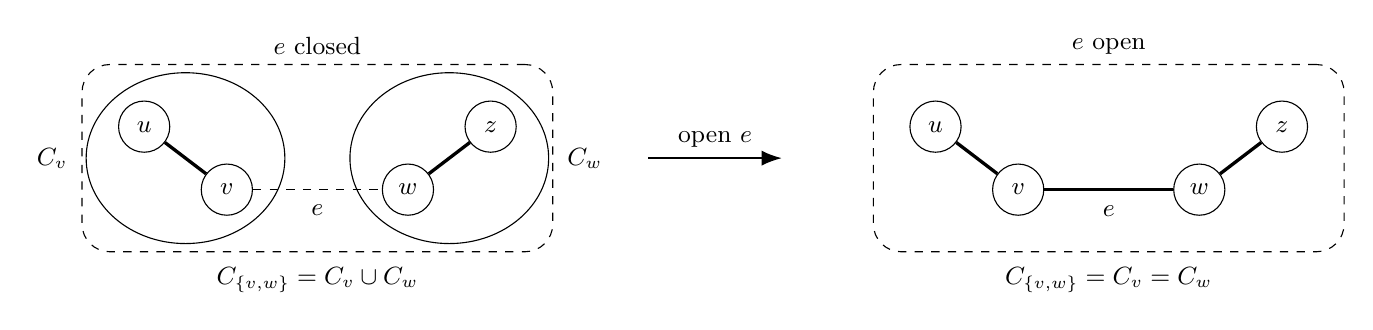
\begin{tikzpicture}[
  vtx/.style={circle,draw,fill=white,inner sep=0pt,minimum size=6.5mm,font=\small},
  open/.style={line width=1.2pt}
]
  \node[vtx] (u0) at (0,0.8)    {$u$};
  \node[vtx] (v0) at (1.05,0)   {$v$};
  \node[vtx] (w0) at (3.35,0)   {$w$};
  \node[vtx] (z0) at (4.4,0.8)  {$z$};
  \draw[open] (u0)--(v0);
  \draw[dashed] (v0)--node[below,font=\small,yshift=-2pt]{$e$}(w0);
  \draw[open] (w0)--(z0);
  \begin{scope}[on background layer]
    \node[draw,ellipse,fit=(u0)(v0),inner sep=1pt] (cv) {};
    \node[draw,ellipse,fit=(w0)(z0),inner sep=1pt] (cw) {};
    \node[draw,dashed,rounded corners=10pt,fit=(u0)(v0)(w0)(z0),inner sep=13pt] (un0) {};
  \end{scope}
  \node[anchor=south,font=\small] at (un0.north) {$e$ closed};
  \node[anchor=east,font=\small]  at (cv.west) [xshift=-3pt] {$C_v$};
  \node[anchor=west,font=\small]  at (cw.east) [xshift=3pt]  {$C_w$};
  \node[anchor=north,font=\small] at (un0.south) [yshift=-2pt] {$C_{\{v,w\}}=C_v\cup C_w$};

  \draw[-{Latex[length=2.6mm]},thick] (6.4,0.4)--node[above,font=\small]{open $e$}(8.1,0.4);

  \node[vtx] (u1) at (10.05,0.8)  {$u$};
  \node[vtx] (v1) at (11.1,0)     {$v$};
  \node[vtx] (w1) at (13.4,0)     {$w$};
  \node[vtx] (z1) at (14.45,0.8)  {$z$};
  \draw[open] (u1)--(v1);
  \draw[open] (v1)--node[below,font=\small,yshift=-2pt]{$e$}(w1);
  \draw[open] (w1)--(z1);
  \begin{scope}[on background layer]
    \node[draw,dashed,rounded corners=10pt,fit=(u1)(v1)(w1)(z1),inner sep=13pt] (un1) {};
  \end{scope}
  \node[anchor=south,font=\small] at (un1.north) {$e$ open};
  \node[anchor=north,font=\small] at (un1.south) [yshift=-2pt] {$C_{\{v,w\}}=C_v=C_w$};
\end{tikzpicture}
\caption{Opening $e$ merges $C_v$ with $C_w$, but the dashed outline, their union
$C_{\{v,w\}}$, is the same in both configurations. On $\{\{v,w\}\ncon a\}$ the cluster
$C_a$ is unchanged as well.}
\label{fig:force-edge}
\end{figure}

\begin{lemma}\label{lem:internal}
Let $v,w\in V$ be distinct, let $e=\{v,w\}$, let $a\in V$, and let $B\subseteq V$.
For a configuration $\omega$ with $e\notin\omega$, write $\omega^e=\omega\cup\{e\}$.
Then
\[
 C_{\{v,w\}}(\omega^e)=C_{\{v,w\}}(\omega).
\]
Consequently, the indicators of $\{\{v,w\}\ncon B\}$ and $\{\{v,w\}\con B\}$ agree in
$\omega$ and $\omega^e$. If $\{v,w\}\ncon a$ in $\omega$, then
$C_a(\omega^e)=C_a(\omega)$.
\end{lemma}

\begin{proof}
Opening $e$ can only enlarge clusters. Conversely, let a simple path in $\omega^e$ join
$v$ or $w$ to $u$. If the path does not use $e$, then it lies in $\omega$. If it uses $e$,
then deleting $e$ leaves a final segment in $\omega$ from one endpoint of $e$ to $u$. Thus
$u\in C_v(\omega)\cup C_w(\omega)$, proving the equality of cluster unions. The two event
identities follow. If $\{v,w\}\ncon a$ in $\omega$, then no path from $a$ in $\omega$ is
connected to either endpoint of $e$, so opening $e$ cannot change $C_a$.
\end{proof}

The next lemma transfers every random variable invariant under the state of $e$ to the
measure in which $e$ is forced open.

\begin{lemma}\label{lem:force}
Let $e$ be an edge and let $\varphi$ be a real function of configurations. Assume
$\varphi(\omega)=\varphi(\omega\cup\{e\})$ for every configuration $\omega$ with
$e\notin\omega$. Then $\EE^e[\varphi]=\EE[\varphi]$.
\end{lemma}

\begin{proof}
Condition on the states of all edges other than $e$. They have the same joint law under
$\PP$ and $\PP^e$, since only $p_e$ differs. Given those states, $\varphi$ has the same
value whether $e$ is open or closed. The conditional expectations, and hence the
unconditional expectations, agree.
\end{proof}

These two invariance facts let us apply Theorem~\ref{thm:fm2} after the edge has been
forced open.

\begin{theorem}\label{thm:c6strong}
Let $A$ be a nonempty finite set of vertices, let $b$ be a vertex, let $a\in A$ satisfy
$\PP(a\con b)\leq\PP(x\con b)$ for every $x\in A$, and let $e=\{v,w\}$ be an edge. Then
\begin{equation}\label{eq:c6strong}
 \PP^e(a\con b,\ v\con A)\leq \PP^e(v\con b,\ v\con A)\,.
\end{equation}
\end{theorem}

\begin{proof}
Apply Theorem~\ref{thm:fm2} with $R=\{v,w\}$ and $F=\one\{b\in\,\cdot\,\}$, for which
$\EE[F(C_x)]=\PP(x\con b)$, so that the hypothesis on $a$ is exactly the minimality assumed
here. Define
\[
 \varphi=(F(C_R)-F(C_a))\one\{R\ncon a,R\con A\setminus\{a\}\}.
\]
Lemma~\ref{lem:internal} shows that both event indicators are invariant under opening $e$.
If $R\ncon a$, both $C_R$ and $C_a$ are invariant; otherwise $\varphi=0$ before and after
opening $e$. Thus $\varphi$ is independent of the state of $e$, and Lemma~\ref{lem:force}
identifies its expectations under $\PP$ and $\PP^e$. Hence
\[
 \EE^e\bigl[F(C_R)-F(C_a);\ R\ncon a,\ R\con A\setminus\{a\}\bigr]\geq 0,\qquad R=\{v,w\}\,.
\]
Under $\PP^e$ the edge $e$ is open with probability one, so almost surely $C_v=C_w=C_R$,
the event $\{R\ncon a\}$ is $\{v\ncon a\}$ and the event $\{R\con A\setminus\{a\}\}$ is
$\{v\con A\setminus\{a\}\}$. Split $\{v\con A\}$ into $\{v\con a\}$, on which $C_v=C_a$ and
the integrand vanishes, and $\{v\ncon a\}\cap\{v\con A\setminus\{a\}\}$. The preceding
restricted expectation is therefore
$\EE^e[\one\{b\in C_v\}-\one\{b\in C_a\};v\con A]\geq0$, which is
\eqref{eq:c6strong}.
\end{proof}

Conjecture~\ref{c6} follows. The events $\{a\con b\}$ and $\{v\con A\}$ are increasing, so
the Harris inequality and \eqref{eq:c6strong} give
\[
 \PP^e(v\con A)\PP^e(a\con b)\leq \PP^e(a\con b,\ v\con A)\leq
 \PP^e(v\con b,\ v\con A)\leq \PP^e(v\con b)\,,
\]
which is \eqref{eq:40}. Its hypothesis \eqref{eq:39} holds automatically: it is the case of
Conjecture~\ref{c1} with $x$ in place of $o$.

\subsection{Starting Vertices}\label{ss:chain}

Throughout this subsection fix a vertex $s$, a set $Y$ of vertices with $s\notin Y$, and an
increasing function $g$ of edge sets, and write $D=\{s\ncon Y\}$. Through Step~7, assume
that every edge probability lies strictly between zero and one. In particular, every
avoidance probability appearing in a denominator below is positive. Step~8 removes this
assumption by continuity. For finite sets $R$,
$X$ and $B$ of vertices put
\[
 H(R;X,B)=\{R\ncon B\}\cap\{R\con X\}\,,
\]
the event that $C_R$ avoids $B$ and meets $X$. The event $\{R\con s\}$ does not imply
$\{R\ncon Y\}$ even when $\{s\ncon Y\}$ holds, because a component of $C_R$ other than the
one containing $s$ may meet $Y$. The two conditions must therefore be carried together. For
a single vertex, however, $H(\{u\};\{s\},Y)=D\cap\{s\con u\}$, since $u\con s$ makes the
clusters of $u$ and $s$ equal. Set
\begin{equation}\label{eq:gamma}
 \Gamma(R)=\PP(D)\,\EE\bigl[g(\eC_s);\,H(R;\{s\},Y)\bigr]
 -\EE\bigl[g(\eC_s);\,D\bigr]\,\PP\bigl(H(R;\{s\},Y)\bigr)\,,
\end{equation}
which at $R=\{u\}$ is $\PP(D)^2$ times the conditional covariance of
Theorem~\ref{thm:csh}. The event $H(R;\{s\},Y)$ is contained in $D$: on it $s$ lies in
$C_R$ and $C_R$ avoids $Y$, so $C_s\subseteq C_R$ avoids $Y$.

The functional \eqref{eq:levels} is now applied to functions of a set argument. Fix
distinct vertices $z_1,\dots,z_\ell$ and a further vertex $v$, all outside $\{s\}\cup Y$
and distinct from each other, and recall the sets $B_j$ of \eqref{eq:constants}. Put
\begin{equation}\label{eq:profile}
 \pi_j(R)=\frac{\PP\bigl(H(R;\{z_j\},B_j)\bigr)}{\PP(z_j\ncon B_j)},\qquad
 \tau(R)=\frac{\PP\bigl(H(R;\{v\},B_{\ell+1})\bigr)}{\PP(v\ncon B_{\ell+1})}\,.
\end{equation}
For a real function $q$ of finite vertex sets put $q^0=q$, then
$q^j(R)=q^{j-1}(R)-\pi_j(R)q^{j-1}(\{z_j\})$ for $1\leq j\leq\ell$, and finally, for a
prescribed set $R_0$,
\begin{equation}\label{eq:margin}
 \Marg[q]=q^\ell(R_0)-\tau(R_0)\,q^\ell(\{v\})\,.
\end{equation}
At a singleton $R_0$ the numbers \eqref{eq:profile} are the constants
\eqref{eq:constants}, and $\Marg[\Gamma]\geq0$ is Theorem~\ref{thm:csh}. The goal of the
first seven steps is the same conclusion for a set $R_0$ with at least two elements.

\medskip\noindent\textbf{Step 1: Linearity.}
There exist real coefficients $(c_u)_{u\in V}$, depending on the percolation law and on the
tuple $(s,Y,z_1,\dots,z_\ell,v,R_0)$ but not on $q$, such that
\[
 \Marg[q]=q(R_0)+\sum_{u\in V}c_uq(\{u\})
\]
for every $q$. This follows by induction on $\ell$: applying the
first subtraction turns $\Marg$ into the functional for $z_2,\dots,z_\ell$ applied to
$R\mapsto q(R)-\pi_1(R)q(\{z_1\})$, and every term the subtraction produces is a multiple
of $q(\{z_1\})$. Only $R_0$ enters with a coefficient not attached to a singleton, and that
coefficient is one. This is what makes the one-sided estimates below usable.

\medskip\noindent\textbf{Step 2: One-Cluster Exploration.}
For a set $U$ of vertices write $\PP_U$ and $\EE_U$ as in Section~\ref{sec:inputs}. Let $X$
be a set of vertices contained in $U$ and containing $s$, let $v\in U\setminus X$, and let
$R\subseteq U$ be disjoint from $X\cup\{v\}$. For vertex sets $B$ and $K$ contained in $U$ put
\begin{equation}\label{eq:alpha}
 \alpha_{R,B}(K)=\one\{K\cap R\neq\varnothing\}\ \PP_{U\setminus K}\bigl(R\setminus K\ncon
 B\bigr)\,.
\end{equation}
Then $\alpha_{R,B}(K)$ is increasing in $K$ and decreasing in $B$, and
\begin{equation}\label{eq:tower}
 \EE_U\bigl[\alpha_{R,B}(C_v);\,v\ncon B\bigr]=\PP_U\bigl(R\ncon B,\ R\con v\bigr)\,.
\end{equation}
The identity follows by summing over the values of $\eC_v$: on $\{v\ncon B\}$ the set
$K=C_v$ is disjoint from $B$, the event $\{R\con v\}$ is
$\{K\cap R\neq\varnothing\}$, and the edges with both endpoints outside $K$ retain their
original probabilities. This argument uses no disjointness hypothesis, so \eqref{eq:tower}
holds for all vertex sets $R$ and $B$ contained in $U$ and every $v\in U$; the placement
hypotheses above are needed only for \eqref{eq:exch1}. Applying
Theorem~\ref{thm:bhk} inside $U$ to the vertex $v$, to the two sets $X\cup N$ and $X\cup
N_1$, and to the functions $\alpha_{R,X\cup N}$ and the constant one, we obtain, for
disjoint $N$ and $N_1$,
\begin{equation}\label{eq:exch1}
 \PP_U\bigl(R\ncon X\cup N,\ R\con v\bigr)\,\PP_U\bigl(v\ncon X\cup N_1\bigr)
\leq \PP_U\bigl(v\ncon X\cup N\cup N_1\bigr)\,\PP_U\bigl(R\ncon X,\ R\con v\bigr)\,.
\end{equation}
Here is the derivation. If $v\in N$ or $v\in N_1$, then one factor on the left of
\eqref{eq:exch1} is zero and there is nothing to prove. Otherwise the two avoided sets
intersect in $X$ and their union is $X\cup N\cup N_1$, so Theorem~\ref{thm:bhk} bounds the
left side by
$\PP_U(v\ncon X\cup N\cup N_1)\,\EE_U[\alpha_{R,X\cup N}(C_v);\,v\ncon X]$. Since
$\alpha_{R,B}$ is decreasing in $B$, the integrand is at most $\alpha_{R,X}(C_v)$, and
\eqref{eq:tower} evaluates the resulting expectation as
$\PP_U(R\ncon X,\ R\con v)$.

\medskip\noindent\textbf{Step 3: Removing Overlap.}
For each set $W\subseteq U$, write
\[
 \varrho(W)=
 \begin{cases}
 \displaystyle
 \frac{\PP_W(R\ncon X,\ R\con v)}{\PP_W(v\ncon X)},
     &\PP_W(v\ncon X)>0,\\[6pt]
 0,&\PP_W(v\ncon X)=0.
 \end{cases}
\]
Let $\eta:2^U\to[0,\infty)$ satisfy $\eta(W)=0$ whenever
$v\notin W$. For sets $Q\subseteq W\subseteq U$, write
\[
 \phi_W(Q)=\EE_W\bigl[\one\{s\ncon Q\}\,\eta(W\setminus C_Q)\bigr]
\]
and
\[
 \Xi_W(Q)=\EE_W\bigl[\one\{s\ncon Q\}\one\{R\ncon Q\}\,
       \varrho(W\setminus C_Q)\eta(W\setminus C_Q)\bigr]\,.
\]
All clusters and probabilities in these expressions are computed in the induced model on
$W$. We abbreviate $\phi_U$ and $\Xi_U$ to $\phi$ and $\Xi$.

The following lemma removes the disjointness assumption in \eqref{eq:exch1}. Its proof is
the only place where we use the Ahlswede--Daykin four functions theorem.

\begin{lemma}\label{lem:overlapavoid}
Let $U$ be a finite set of vertices. Let $s,v\in U$, and let $X,R,N,N_1\subseteq U$ satisfy
$s\in X$, $v\notin X$, and $R\cap(X\cup\{v\})=\varnothing$. Let
$\eta:2^U\to[0,\infty)$ satisfy $\eta(W)=0$ whenever $v\notin W$. For
$Q\subseteq W\subseteq U$, define
\[
 \varrho(W)=
 \begin{cases}
 \PP_W(R\ncon X,R\con v)/\PP_W(v\ncon X),&\PP_W(v\ncon X)>0,\\
 0,&\PP_W(v\ncon X)=0,
 \end{cases}
\]
\[
 \phi_W(Q)=\EE_W[\one\{s\ncon Q\}\eta(W\setminus C_Q)],
\]
\[
 \Xi_W(Q)=\EE_W[\one\{s\ncon Q\}\one\{R\ncon Q\}
 \varrho(W\setminus C_Q)\eta(W\setminus C_Q)].
\]
Write $\phi=\phi_U$ and $\Xi=\Xi_U$. Assume that for every $W\subseteq U$ containing $s$
and $v$, both of the following hold: the map $Q\mapsto\phi_W(Q)$ is decreasing, and
\begin{equation}\label{eq:stopped-general}
 \phi_W(Q)\,\PP_W(v\ncon X)
 \leq \PP_W(v\ncon X\cup Q)\,\eta(W)
\end{equation}
for every $Q\subseteq W$. Then
\begin{equation}\label{eq:twosource}
 \PP_U\bigl(R\ncon X\cup N,\ R\con v\bigr)\,\phi(N_1)
 \leq \PP_U\bigl(v\ncon X\cup N\cup N_1\bigr)\,\Xi(N\cap N_1)\,.
\end{equation}
\end{lemma}

\begin{proof}
We use strong induction on $|U|$. Suppose first that $N\cap N_1=\varnothing$.
Inequality~\eqref{eq:stopped-general}, applied with $W=U$ and $Q=N_1$, gives
\[
 \phi(N_1)\PP_U(v\ncon X)
 \leq \PP_U(v\ncon X\cup N_1)\eta(U)\,.
\]
Inequality~\eqref{eq:exch1} gives
\[
 \PP_U(R\ncon X\cup N,R\con v)\PP_U(v\ncon X\cup N_1)
 \leq
 \PP_U(v\ncon X\cup N\cup N_1)\PP_U(R\ncon X,R\con v)\,.
\]
Multiply these inequalities. If $\PP_U(v\ncon X)>0$, divide by this probability and use
$\Xi(\varnothing)=\varrho(U)\eta(U)$ to obtain \eqref{eq:twosource}. If
$\PP_U(v\ncon X)=0$, then
\[
 \PP_U(R\ncon X\cup N,R\con v)
 \leq \PP_U(v\ncon X\cup N)
 \leq \PP_U(v\ncon X)=0\,.
\]
The left side of \eqref{eq:twosource} therefore vanishes in the zero-denominator case.

Now suppose that $Z=N\cap N_1$ is nonempty. The left side again vanishes if $v\in Z$, if
$s\in Z$, or if $R\cap Z$ is nonempty. We may therefore assume that $Z$ is disjoint from
$R\cup\{s,v\}$. Put $U_0=U\setminus Z$ and $X_0=X\cap U_0$.

Expose all edges with exactly one endpoint in $Z$, and let $S\subseteq U_0$ consist of the
vertices joined to $Z$ by at least one exposed open edge. The events determining
membership in $S$ use disjoint edge families as the vertex varies. Thus $S$ has a product law; write
$\mu_Z$ for its mass function. For all $S_1,S_2\subseteq U_0$,
\begin{equation}\label{eq:product-neighbour-law}
 \mu_Z(S_1)\mu_Z(S_2)
 =\mu_Z(S_1\cap S_2)\mu_Z(S_1\cup S_2)\,.
\end{equation}

For $S\subseteq U_0$, write
\[
 \begin{aligned}
 E(S)&=\PP_{U_0}\bigl(R\ncon X_0\cup(N\setminus Z)\cup S,\ R\con v\bigr),\\
 L(S)&=\phi_{U_0}\bigl((N_1\setminus Z)\cup S\bigr),\\
 M(S)&=\PP_{U_0}\bigl(v\ncon
       X_0\cup(N\setminus Z)\cup(N_1\setminus Z)\cup S\bigr),\\
 K(S)&=\Xi_{U_0}(S).
 \end{aligned}
\]
The domain Markov property gives four exact identities:
\[
 \begin{aligned}
 \PP_U(R\ncon X\cup N,R\con v)&=\sum_{S\subseteq U_0}\mu_Z(S)E(S),\\
 \phi_U(N_1)&=\sum_{S\subseteq U_0}\mu_Z(S)L(S),\\
 \PP_U(v\ncon X\cup N\cup N_1)&=\sum_{S\subseteq U_0}\mu_Z(S)M(S),\\
 \Xi_U(Z)&=\sum_{S\subseteq U_0}\mu_Z(S)K(S).
 \end{aligned}
\]
These formulas express the four quantities in the percolation model on the smaller vertex
set $U_0$.

It remains to verify the pointwise hypothesis of the four functions theorem. Fix
$S_1,S_2\subseteq U_0$, and put
\[
 Q=S_1\cup\bigl((N\setminus Z)\setminus S_2\bigr),\qquad
 Q_1=S_2\cup\bigl((N_1\setminus Z)\setminus S_1\bigr)\,.
\]
Avoidance is decreasing in the avoided set, and $Q\mapsto\phi_{U_0}(Q)$ is decreasing.
Hence
\[
 E(S_1)\leq\PP_{U_0}(R\ncon X_0\cup Q,R\con v),
 \qquad L(S_2)\leq\phi_{U_0}(Q_1)\,.
\]
Because $Z=N\cap N_1$, the two constructed sets satisfy
\[
 Q\cup Q_1=(N\setminus Z)\cup(N_1\setminus Z)\cup S_1\cup S_2,
 \qquad Q\cap Q_1=S_1\cap S_2\,.
\]
The induction hypothesis in $U_0$ therefore yields
\begin{equation}\label{eq:four-pointwise}
 E(S_1)L(S_2)\leq M(S_1\cup S_2)K(S_1\cap S_2)\,.
\end{equation}
For $W\subseteq U_0$, every vertex of $X\setminus X_0$ lies outside the induced model and
is isolated. Hence the events $\{v\ncon X\}$ and $\{v\ncon X_0\}$, and their unions with
$Q$, coincide under $\PP_W$. This transfers \eqref{eq:stopped-general} to the smaller
problem. Nonnegativity, the vanishing condition for $\eta$, and the monotonicity of
$\phi_W$ restrict directly to $U_0$.

Apply the Ahlswede--Daykin four-functions theorem to
\[
 \mu_Z(S)E(S),\qquad \mu_Z(S)L(S),\qquad
 \mu_Z(S)M(S),\qquad \mu_Z(S)K(S)\,.
\]
The pointwise hypothesis follows from \eqref{eq:four-pointwise} and
\eqref{eq:product-neighbour-law}. The four exact identities then turn its conclusion into
\eqref{eq:twosource}. This completes the strong induction.
\end{proof}

This proves the required comparison when the two extra avoided sets overlap. We will use
it after exposing $C_Y$, where the two avoided sets are equal.

\medskip\noindent\textbf{Step 4: One-Vertex Comparison.}
Let $\eta_R(U)=\Cov_U(g(\eC_s),\one\{R\con X\})$ and let $\eta_v(U)$ be as in
\eqref{eq:etadef}. Then $\eta_v(U)\geq0$ and
\begin{equation}\label{eq:fourpoint}
 \varrho(U)\,\eta_v(U)\leq \eta_R(U)\,.
\end{equation}
Write $J$ for $\{R\ncon X\}\cap\{R\con v\}$. The union of $\{R\con X\}$ and $J$ is
increasing, so Harris gives $\eta_R\geq\EE_U[g(\eC_s)]\PP_U(J)-\EE_U[g(\eC_s);J]$. The
function $g(\eC_s)$ is increasing in $\eC_X$ and does not depend on $\eC_v$, while $\one_J$
is decreasing in $\eC_X$ and increasing in $\eC_v$. Hence \eqref{eq:bhkneg} with $S_1=X$ and
$S_2=\{v\}$ gives $\PP_U(v\ncon X)\EE_U[g(\eC_s);J]\leq\PP_U(J)\EE_U[g(\eC_s);v\ncon X]$,
and substituting the definitions gives \eqref{eq:fourpoint}.

\medskip\noindent\textbf{Step 5: Exposing $C_Y$.}
Let $X=\{s\}\cup\{z_1,\dots,z_\ell\}$, let $v$ lie outside $X\cup Y$, and let $R_0$ be
disjoint from $X\cup Y\cup\{v\}$. Write $U=V\setminus C_Y$ and
\[
 \mathcal H\coloneqq\EE\bigl[\one_D\one\{R_0\ncon Y\}\,\eta_{R_0}(U)\bigr]
 -\tau(R_0)\,\EE\bigl[\one_D\,\eta_v(U)\bigr]\,.
\]
$\mathcal H$ is nonnegative. Indeed, for every $W\subseteq V$ and $Q\subseteq W$, the
stopped-covariance estimate gives
\[
 \phi_W(Q)\PP_W(v\ncon X)\leq
 \PP_W(v\ncon X\cup Q)\eta_v(W),
\]
and $Q\mapsto\phi_W(Q)$ is decreasing. Thus Lemma~\ref{lem:overlapavoid} applies with
$U=V$, $R=R_0$, $N=N_1=Y$, and $\eta=\eta_v$. Since $B_{\ell+1}=X\cup Y$, the ratio
$\PP(H(R_0;\{v\},X\cup Y))/\PP(v\ncon X\cup Y)$ is $\tau(R_0)$. Dividing by the positive
denominator gives
$\tau(R_0)\EE[\one_D\eta_v(U)]\leq
\EE[\one_D\one\{R_0\ncon Y\}\varrho(U)\eta_v(U)]$.
Inequality~\eqref{eq:fourpoint} inside $U$ bounds the integrand on the right.

\medskip\noindent\textbf{Step 6: Exposing $C_R$.}
Let $z$ be a vertex and let $B$ contain $\{s\}\cup Y$ but not $z$, and abbreviate
$H_R=H(R;\{z\},B)$ and $E=\{z\ncon B\}$, with $\PP(E)>0$. Summing over the values of
$\eC_R$ gives $\EE[\Theta;H_R]=-\EE[\Psi(C_R);H_R]$: on $H_R$ the set $C_R$ is disjoint
from $B$ and every edge with exactly one endpoint in $C_R$ is closed, so the conditional expectation of
$\Theta$ is $-\Psi(C_R)$. On $H_R$ at least one vertex of $R$ is joined to $z$, so
$C_z\subseteq C_R$, and therefore
\[
 \Delta(R)=\EE\bigl[\Psi(C_R)-\Psi(C_z);H_R\bigr]\geq 0\,,
\]
with $\Delta(\{u\})=0$ for every vertex $u$, since $C_{\{u\}}=C_z$ on $H_{\{u\}}$. Set
\[
\begin{split}
 \Gamma_{z,B}(Q)
 &=\PP(z\ncon B)\,
   \EE[\Psi(C_z);H(Q;\{z\},B)]\\
 &\quad-\EE[\Psi(C_z);z\ncon B]\,
   \PP(H(Q;\{z\},B)).
\end{split}
\]
This is \eqref{eq:gamma} with $s=z$, avoided set $B$, and
$g(K)=\Psi(\{z\}\cup\vtx K)$. Expanding $\Gamma_{z,B}$, then using the
displayed identity, the definition of $\Delta$ and \eqref{eq:markov1}, gives
\begin{equation}\label{eq:cgdi}
 \EE[\Theta;H_R]-\pi(R)\,\EE[\Theta;E]=-\frac{\Gamma_{z,B}(R)}{\PP(E)}-\Delta(R),
 \qquad \pi(R)=\frac{\PP(H_R)}{\PP(E)}\,,
\end{equation}
and hence, dropping $\Delta(R)\geq0$,
\[
 \EE[\Theta;H_R]-\pi(R)\,\EE[\Theta;E]\leq -\frac{\Gamma_{z,B}(R)}{\PP(E)}\,,
\]
with equality whenever $R$ is a single vertex.

\medskip\noindent\textbf{Step 7: Auxiliary Vertices.}
For each increasing function $q$ of edge sets, let
$\Theta_q,\Psi_q,\mathcal H(q),\Gamma^q_{z,B}$, and $\Delta^q_{z,B}$ denote the quantities
defined in \eqref{eq:resid} and Steps~5--6 with $g$ replaced by $q$. Without subscripts,
$\Gamma^q$ denotes the function in \eqref{eq:gamma} with starting vertex $s$, avoided set
$Y$, and $g=q$. Put
\[
 \mathcal W(q)=\EE\Bigl[\Theta_q\,
   \Marg\bigl[R\mapsto\one_{H(R;\{s\},Y)}\bigr]\Bigr],
\]
where $\Marg$ acts on the argument $R$ while $\eC_s$ and $\eC_Y$ are held fixed. For
$1\leq j\leq\ell$, let $\Marg_j$ be the functional formed from
$z_{j+1},\ldots,z_\ell$, from $v$, and from $R_0$, with base avoided set $B_{j+1}$. In
the term indexed by $j$, let $\Gamma^q_{z_j,B_j}$ be \eqref{eq:gamma} formed with the
increasing function
\[
 K\longmapsto\Psi_q(\{z_j\}\cup\vtx K).
\]
Let $\Delta^q_j(R)$ be the quantity $\Delta(R)$ in Step~6 with $z=z_j$, $B=B_j$, and
$\Psi=\Psi_q$.

Apply \eqref{eq:cgdi} first at $z_1$, then at $z_2$, and continue through $z_\ell$.
Linearity of $\Marg$ gives
\begin{equation}\label{eq:unfold}
 \mathcal W(q)=\mathcal H(q)
 +\sum_{j=1}^{\ell}\frac{\Marg_j\bigl[\Gamma^q_{z_j,B_j}\bigr]}{\PP(z_j\ncon B_j)}
 +\sum_{j=1}^{\ell}\Delta^q_j(R_0)\,.
\end{equation}
At the $j$th subtraction, \eqref{eq:cgdi} produces one covariance with the shorter list
and one copy of $\Delta^q_j$. Step~1 writes the remaining functional as evaluation at
$R_0$, with coefficient one, plus evaluations at singletons. Because $\Delta^q_j$
vanishes at every singleton, only $\Delta^q_j(R_0)$ remains. The term depending only on
$\eC_Y$ has zero expectation because $\EE[\Theta_q\mid\eC_Y]=0$. After the last
subtraction, the remaining term is $\mathcal H(q)$, proving \eqref{eq:unfold}.

We next pass from $\mathcal W(q)$ to the covariance in \eqref{eq:gamma}. For possible
values $K_s$ and $K_Y$ of $\eC_s$ and $\eC_Y$, respectively, define
\[
 h(K_s,K_Y)=
 \Marg\!\left[
 R\mapsto
 \one\!\left\{
 R\cap(\{s\}\cup\vtx K_s)\neq\varnothing,\
 R\cap(Y\cup\vtx K_Y)=\varnothing
 \right\}\right].
\]
If $K_Y\subseteq L_Y$, then $h(K_s,L_Y)\leq h(K_s,K_Y)$. Indeed, the term evaluated at
$R_0$ requires $R_0$ to avoid the larger cluster represented by $L_Y$. Each singleton
term is independent of the second argument because, on $D=\{s\ncon Y\}$, a vertex
connected to $s$ cannot also be connected to $Y$.

For an increasing function $q$ of edge sets, put
\[
 \mathcal V(q)=\PP(D)\,
   \EE\bigl[q(\eC_s)h(\eC_s,\eC_Y);D\bigr]
 -\EE\bigl[q(\eC_s);D\bigr]\,
  \EE\bigl[h(\eC_s,\eC_Y);D\bigr].
\]
Thus $\mathcal V(q)$ is the unnormalized covariance under $\PP(\,\cdot\mid D)$. By
definition, it equals $\Marg[\Gamma^q]$.

We now define the alternating conditional-expectation operator used below. Let
$\nu=\PP(\,\cdot\mid D)$ and, for every value $L$ of $\eC_Y$ in the support of $\nu$, set
\[
 Q_q(L)=\EE_\nu[q(\eC_s)\mid\eC_Y=L].
\]
For every value $K$ of $\eC_s$ in the support of $\nu$, define
\begin{equation}\label{eq:gibbs-operator}
 (\mathcal Kq)(K)=\EE_\nu[Q_q(\eC_Y)\mid\eC_s=K].
\end{equation}
This finite-state formula first applies conditional expectation given $\eC_Y$ and then
conditional expectation given $\eC_s$; it determines $\mathcal K$ without choosing
versions on null states.

Define the reverse conditional-covariance term by
\[
 \mathcal W_2(q)=\PP(D)\,
 \EE_\nu\!\left[
 \Cov_\nu\!\left(Q_q(\eC_Y),h(\eC_s,\eC_Y)\mid\eC_s\right)\right].
\]
The definition of $\Theta_q$ gives
\[
 \mathcal W(q)=\PP(D)\,
 \EE_\nu\!\left[
 \Cov_\nu\!\left(q(\eC_s),h(\eC_s,\eC_Y)\mid\eC_Y\right)\right].
\]
Twice applying the law of total covariance, or directly expanding the finite sums, yields
\begin{equation}\label{eq:two-cluster-step}
 \mathcal V(q)-\mathcal V(\mathcal Kq)
 =\PP(D)\bigl(\mathcal W(q)+\mathcal W_2(q)\bigr).
\end{equation}

If $q$ is increasing, then
\[
 L\longmapsto\EE_\nu[q(\eC_s)\mid\eC_Y=L]
\]
is decreasing: enlarging the exposed cluster of $Y$ closes more edges available to
$C_s$. The function $L\mapsto h(K,L)$ is also decreasing. Conditional positive
association therefore gives $\mathcal W_2(q)\geq0$. The same cluster-exploration coupling
shows that $\mathcal Kq$ is increasing. Consequently, once $\mathcal W(q)\geq0$ is known
for every increasing $q$, \eqref{eq:two-cluster-step} gives
\[
 \mathcal V(\mathcal Kq)\leq\mathcal V(q).
\]

It remains to show that this monotonicity forces $\mathcal V(q)\geq0$. For a function on a
finite state space, write $\operatorname{osc}(q)=\max q-\min q$. Set
\[
 \varepsilon=\prod_{e:\,e\cap Y\neq\varnothing}(1-p_e)>0,
 \qquad \beta=1-\varepsilon<1.
\]
During the first conditional draw in \eqref{eq:gibbs-operator}, all edges meeting $Y$ are
closed with conditional probability at least $\varepsilon$. On that event
$\eC_Y=\varnothing$, and the law of the second draw of $\eC_s$ is independent of the
initial value $K$. Thus every transition law of $\mathcal K$ has a common component of
mass at least $\varepsilon$, and the elementary coupling bound gives
\[
 \operatorname{osc}(\mathcal K^nq)\leq
 \beta^n\operatorname{osc}(q).
\]
If $H_0$ is the largest value of $|h(K,L)|$ over the pairs $(K,L)$ of values that
$(\eC_s,\eC_Y)$ takes with positive probability under $\nu$, then
\[
 |\mathcal V(\mathcal K^nq)|
 \leq2\PP(D)^2H_0\,\operatorname{osc}(\mathcal K^nq)
 \leq2H_0\beta^n\operatorname{osc}(q).
\]
Iteration gives $\mathcal V(\mathcal K^nq)\leq\mathcal V(q)$, while the displayed bound
tends to zero. Hence $\mathcal V(q)\geq0$.

We can now close the strong induction on $\ell$. We prove simultaneously, for every
increasing $q$, that $\mathcal W(q)\geq0$ and $\Marg[\Gamma^q]\geq0$. If $\ell=0$, then
\eqref{eq:unfold} reduces to $\mathcal W(q)=\mathcal H(q)$. Step~5 gives
$\mathcal H(q)\geq0$, and the preceding covariance argument gives
$\Marg[\Gamma^q]\geq0$.

For the inductive step, suppose both conclusions hold for all shorter lists. The term
$\mathcal H(q)$ in \eqref{eq:unfold} is nonnegative by Step~5. Each denominator
$\PP(z_j\ncon B_j)$ is positive because closing all edges incident to $z_j$ forces
$z_j\ncon B_j$ and has positive probability. The function used in
$\Gamma^q_{z_j,B_j}$ is increasing, and its auxiliary list is
$z_{j+1},\ldots,z_\ell$. The induction hypothesis gives
$\Marg_j[\Gamma^q_{z_j,B_j}]\geq0$. Step~6 gives $\Delta^q_j(R_0)\geq0$. Every term on the
right side of \eqref{eq:unfold} is therefore nonnegative, so $\mathcal W(q)\geq0$. The
covariance argument then gives $\Marg[\Gamma^q]\geq0$ at length $\ell$. The first conclusion
at length $\ell$ uses only the second conclusion for shorter lists, while the second uses
the first at the current length. Thus the induction is not circular.

\medskip\noindent\textbf{Step 8: Induction on $T$.}
Recall $Y$, $F$, $T$, $r$, and the numbers $m_x$ of Section~\ref{sec:gen}. For a finite set
$R$ of vertices put
\[
 J_x(R)=\{R\ncon Y\}\cap\{R\con x\}\cap\bigcap_{y\in T,\ r(y)<r(x)}\{R\ncon y\},
\]
\[
 \Lambda_R(T)=\EE\bigl[F(C_R);\,R\ncon Y,\ R\con T\bigr]
 -\sum_{x\in T}\PP\bigl(J_x(R)\bigr)\,m_x\,.
\]
For $R=\{u\}$ these are \eqref{eq:pattern} and \eqref{eq:surplus}.

We can now prove the version of Theorem~\ref{thm:gen} with a finite starting set.

\begin{theorem}\label{thm:pairgen}
Let $V$ be a finite vertex set with edge probabilities in $[0,1]$. Let $Y,R\subseteq V$,
and let $T\subseteq V\setminus Y$ be finite. Assume that $R$ is nonempty and disjoint from
$Y\cup T$. Let $F$ be an increasing real function on the subsets of $V$, and assume
$\PP(x\ncon Y)>0$ for every $x\in T$. For each $x\in T$, let
\[
 m_x=\frac{\EE[F(C_x);\,x\ncon Y]}{\PP(x\ncon Y)}\,.
\]
Let $r$ be an injective real function on $T$ such that $m_x\leq m_y$ whenever
$r(x)<r(y)$. For $x\in T$, define
\[
 J_x(R)=\{R\ncon Y,R\con x\}\cap
 \bigcap_{\substack{y\in T\\r(y)<r(x)}}\{R\ncon y\},
\]
and set
\[
 \Lambda_R(T)=\EE[F(C_R);R\ncon Y,R\con T]
 -\sum_{x\in T}\PP(J_x(R))m_x.
\]
Then $\Lambda_R(T)\geq0$.
\end{theorem}

\begin{proof}
If $R$ is a singleton, then the conclusion is Theorem~\ref{thm:gen}. Assume first that $R$ has
at least two elements and that every edge probability lies strictly between zero and one.
We use two inductions. The first establishes the transfer estimate
\eqref{eq:source-margin}, which is used in the main induction.

For each $S\subseteq T$, let $\mathsf P(S)$ assert that the inequality
\[
 \Marg\bigl[\,Q\mapsto\Lambda_Q(S)\,\bigr]\geq0
\]
holds for every nonempty $R$ with
$|R|\geq2$ and $R\cap(Y\cup S)=\varnothing$, every length $\ell$, every pairwise distinct
list $z_1,\ldots,z_\ell$ outside $R\cup Y\cup S$, and every vertex $v$ outside
$R\cup Y\cup S\cup\{z_1,\ldots,z_\ell\}$. In this
definition, $\Marg$ is given by \eqref{eq:profile}--\eqref{eq:margin} with initial
avoided set $B_1=Y\cup S$. We prove $\mathsf P(S)$ by induction on $|S|$. Thus, for the
current set $T$, the conclusion is
\begin{equation}\label{eq:source-margin}
 \Marg\bigl[Q\mapsto\Lambda_Q(T)\bigr]\geq0\,.
\end{equation}
The claim is immediate for $S=\varnothing$. For the inductive step, fix
$R,z_1,\ldots,z_\ell,v$ satisfying these conditions, choose $k\in S$ with maximal
$r(k)$, and write
$S_0=S\setminus\{k\}$. Then $m_x\leq m_k$ for every $x\in S_0$.
Write
\[
 E_k=\{k\ncon Y\cup S_0\},\qquad
 G_k(Q)=H(Q;\{k\},Y\cup S_0),\qquad d_k=\PP(E_k),
\]
and define
\[
 K_k(Q)=\EE[F(C_k)-m_k;\,G_k(Q)],\qquad
 c_k(Q)=\frac{\PP(G_k(Q))}{d_k},
\]
\[
 \kappa_k=m_kd_k-\EE[F(C_k);E_k]\,.
\]
The all-closed configuration belongs to $E_k$, so $d_k>0$.

Adding the vertex $k$, whose value $r(k)$ is maximal, to $S_0$ gives
\[
 \Lambda_Q(S)=\Lambda_Q(S_0)
   +\EE[F(C_Q)-m_k;\,G_k(Q)]\,.
\]
On $G_k(Q)$ we have $C_k\subseteq C_Q$. Monotonicity of $F$ therefore gives the lower
bound
\[
 \Lambda_Q(S)\geq\Lambda_Q(S_0)+K_k(Q),
\]
with equality whenever $Q$ is a singleton. Step~1 now gives
\begin{equation}\label{eq:source-peel-margin}
 \Marg[\Lambda_\cdot(S)]
 \geq \Marg[\Lambda_\cdot(S_0)+K_k]\,.
\end{equation}

Let $g_k(K)=F(\{k\}\cup\vtx K)$ and define
\[
 \Gamma_k(Q)=d_k\EE[g_k(\eC_k);G_k(Q)]
 -\EE[g_k(\eC_k);E_k]\PP(G_k(Q)).
\]
This is \eqref{eq:gamma} with starting vertex $k$ and avoided set $Y\cup S_0$. Direct
expansion gives, for every vertex set $Q$,
\begin{equation}\label{eq:source-kappa-covariance}
 d_kK_k(Q)=\Gamma_k(Q)-\kappa_kd_kc_k(Q)\,.
\end{equation}
Step~7 gives $\Marg[\Gamma_k]\geq0$. For the second application, set
$h_k(K)=\one\{K\neq\varnothing\}$ and
$q_k=\PP(E_k,\eC_k=\varnothing)>0$. At every set $Q$ where $\Marg$ evaluates a function,
$k\notin Q$; hence $G_k(Q)$ implies $\eC_k\neq\varnothing$. The version of $\Gamma_k$
formed with $h_k$ is therefore
\[
 d_k\PP(G_k(Q))-(d_k-q_k)\PP(G_k(Q))
 =q_kd_kc_k(Q).
\]
Step~7 gives $q_kd_k\Marg[c_k]\geq0$, and thus $\Marg[c_k]\geq0$.

Partitioning $\{k\ncon Y\}$ according to the first vertex of $S_0$ connected to $k$ gives
\begin{equation}\label{eq:source-repricing}
 \Lambda_{\{k\}}(S_0)-\kappa_k
 =\sum_{x\in S_0}\PP(J_x(\{k\}))(m_k-m_x)\geq0\,.
\end{equation}
The induction hypothesis for $S_0$, with $k$ inserted before
$z_1,\ldots,z_\ell$ in the auxiliary list, is
\[
 \Marg[\Lambda_\cdot(S_0)]
 -\Lambda_{\{k\}}(S_0)\Marg[c_k]\geq0\,.
\]
Combining \eqref{eq:source-peel-margin}, \eqref{eq:source-kappa-covariance},
\eqref{eq:source-repricing}, and the inserted-list induction hypothesis gives
\[
\begin{aligned}
 d_k\Marg[\Lambda_\cdot(S)]
 &\geq d_k\Marg[\Lambda_\cdot(S_0)+K_k]\\
 &=d_k\Marg[\Lambda_\cdot(S_0)]
   +\Marg[\Gamma_k]-\kappa_kd_k\Marg[c_k]\\
 &\geq d_k\bigl(\Marg[\Lambda_\cdot(S_0)]
   -\Lambda_{\{k\}}(S_0)\Marg[c_k]\bigr)
   +\Marg[\Gamma_k]\geq0.
\end{aligned}
\]
Since $d_k>0$, this proves \eqref{eq:source-margin}.

Apply \eqref{eq:source-margin} to $S_0$, with no auxiliary vertices and with comparison
vertex $k$. The definition of $\Marg$ gives
\begin{equation}\label{eq:pairtransfer}
 \PP\bigl(G_k(R)\bigr)\Lambda_{\{k\}}(S_0)
 \leq d_k\Lambda_R(S_0)\,.
\end{equation}

We now prove $\Lambda_R(T)\geq0$ by induction on $|T|$. The claim is immediate for
$T=\varnothing$. For the inductive step, choose $k\in T$ with maximal $r(k)$, put
$T_0=T\setminus\{k\}$, and define
\[
 E_k=\{k\ncon Y\cup T_0\},\quad
 G_k(R)=H(R;\{k\},Y\cup T_0),\quad d_k=\PP(E_k),
\]
\[
 \kappa_k=m_kd_k-\EE[F(C_k);E_k].
\]
Also put
\[
 I_k=\EE[F(C_R)-m_k;\,G_k(R)]\,.
\]
The exact decomposition after adjoining $k$ is
\[
 \Lambda_R(T)=\Lambda_R(T_0)+I_k\,.
\]
We next estimate $I_k$. Under the conditional law on $E_k$, apply positive association
to the increasing random variables
\[
 F(C_k)\quad\text{and}\quad \alpha_{R,Y\cup T_0}(C_k).
\]
The identity
\eqref{eq:tower}, first alone and then with the factor $F(C_k)$, gives
\[
 \EE[\alpha_{R,Y\cup T_0}(C_k);E_k]=\PP(G_k(R))
\]
and
\[
 \EE[F(C_k)\alpha_{R,Y\cup T_0}(C_k);E_k]
   =\EE[F(C_k);G_k(R)]\,.
\]
Conditional positive association gives
\[
 d_k\EE[F(C_k);G_k(R)]
 \geq \EE[F(C_k);E_k]\PP(G_k(R)).
\]
Because $C_k\subseteq C_R$ on $G_k(R)$, monotonicity of $F$ then gives
\[
 d_k I_k\geq-\PP(G_k(R))\kappa_k\,.
\]
By \eqref{eq:source-repricing}, $\kappa_k\leq\Lambda_{\{k\}}(T_0)$. Therefore
\[
\begin{aligned}
 d_k\Lambda_R(T)
 &=d_k\Lambda_R(T_0)+d_kI_k\\
 &\geq d_k\Lambda_R(T_0)-\PP(G_k(R))\kappa_k\\
 &\geq d_k\Lambda_R(T_0)
   -\PP(G_k(R))\Lambda_{\{k\}}(T_0)\geq0,
\end{aligned}
\]
where the last inequality is \eqref{eq:pairtransfer}. Dividing by $d_k>0$ completes the
induction for edge probabilities strictly between zero and one.

It remains to allow edge probabilities equal to zero or one. For every injective $r$
satisfying $m_x\leq m_y$ whenever $r(x)<r(y)$, the partition by the first connected
vertex gives
\[
 \Lambda_R(T)=\EE\!\left[
 \one\{R\ncon Y,\ R\con T\}
 \left(F(C_R)-\min_{x\in T\cap C_R}m_x\right)\right].
\]
This expression is independent of the order used to break ties. It depends continuously
on the edge probabilities whenever $\PP(x\ncon Y)>0$ for every $x\in T$. Approximate the
given probabilities by probabilities in the open unit interval, and for each approximation
choose an injective $r$ ordered by its corresponding values $m_x$. The interior case
applies to every approximation, so continuity gives $\Lambda_R(T)\geq0$ at the original
probabilities.
\end{proof}

\medskip\noindent\textbf{Step 9: Removing the Conditioning.}
An identity and a comparison relate $F$ to $\Phi_a$ when several vertices replace one. Let $R$
be a nonempty finite set of vertices, let $a$ be a vertex and let $\mathcal S$ be a family
of edge sets.

\begin{lemma}\label{lem:projset}
For every nonempty set $R$, every vertex $a$, every increasing function $F$ of vertex
sets, and every family $\mathcal S$ of edge sets,
\begin{equation}\label{eq:projset}
 \EE\bigl[F(C_R)-F(C_a);\ R\ncon a,\ \eC_R\in\mathcal S\bigr]
 =\EE\bigl[\Phi_a(C_R);\ R\ncon a,\ \eC_R\in\mathcal S\bigr]\,.
\end{equation}
\end{lemma}

\begin{proof}
Condition on $\eC_R$. On $\{R\ncon a\}$ the vertex $a$ lies outside $C_R$, every edge
with exactly one endpoint in $C_R$ is closed, and the edges with both endpoints outside
$C_R$ retain their original probabilities. The conditional expectation of $F(C_a)$ is
therefore the expectation subtracted from $F(C_R)$ in the definition of $\Phi_a(C_R)$.
Both $\{R\ncon a\}$ and $\{\eC_R\in\mathcal S\}$ are determined by $\eC_R$. Summing over
the possible values of $\eC_R$ proves \eqref{eq:projset}.
\end{proof}

The next lemma handles the case where the starting set already contains a vertex whose
unconditional mean is at least that of $a$.

\begin{lemma}\label{lem:overlap}
Let $R$ be a nonempty set of vertices, let $a$ be a vertex, and let $F$ be an increasing
function of vertex sets. If there is a vertex $s\in R$ such that
$\EE[F(C_a)]\leq\EE[F(C_s)]$, then
\begin{equation}\label{eq:overlap}
 \EE\bigl[F(C_R)-F(C_a);\ R\ncon a\bigr]\geq 0\,.
\end{equation}
\end{lemma}

\begin{proof}
For $K=C_s$, the function in \eqref{eq:alpha} is
\[
 \alpha_{R,\{a\}}(C_s)
 =\PP_{V\setminus C_s}(R\setminus C_s\ncon a)
\]
on $\{s\ncon a\}$, because $s\in R\cap C_s$. It is increasing, and
\eqref{eq:tower} gives
\[
 \EE[\Phi_a(C_s);R\ncon a]
 =\EE[\Phi_a(C_s)\alpha_{R,\{a\}}(C_s);s\ncon a].
\]
Apply \eqref{eq:bhk1} with
vertex $s$, with $X=\{a\}$ and with the two increasing functions
$\eC\mapsto\Phi_a(\{s\}\cup\vtx\eC)$ and $\eC\mapsto\alpha_{R,\{a\}}(\{s\}\cup\vtx\eC)$.
Lemma~\ref{lem:proj}(ii) gives
\[
 \EE[\Phi_a(C_s);s\ncon a]
 =\EE[F(C_s)]-\EE[F(C_a)]\geq0.
\]
If $\PP(s\ncon a)=0$, then $\{R\ncon a\}\subseteq\{s\ncon a\}$ because $s\in R$, so
$\{R\ncon a\}$ is null and the expectation in \eqref{eq:overlap} is zero. Assume therefore
that $\PP(s\ncon a)>0$. Since the other factor in \eqref{eq:bhk1} is nonnegative, the
preceding identity gives $\PP(s\ncon a)\,\EE[\Phi_a(C_s);R\ncon a]\geq0$, and division by
$\PP(s\ncon a)$ gives $\EE[\Phi_a(C_s);R\ncon a]\geq0$. On $\{R\ncon a\}$, the inclusion
$C_s\subseteq C_R$ and monotonicity of $\Phi_a$ imply
$\EE[\Phi_a(C_R);R\ncon a]\geq0$. Equation~\eqref{eq:projset} now gives
\eqref{eq:overlap}.
\end{proof}

\begin{proof}[Proof of Theorem~\ref{thm:fm2}]
Put $T=A\setminus\{a\}$. If $a\in R$, then $\{R\ncon
a\}$ is empty and the restricted expectation in \eqref{eq:fm2} is zero. If
$R\cap T\neq\varnothing$, choose $s\in R\cap T$; then $\{R\con T\}$ occurs surely and
\eqref{eq:overlap} applies. Otherwise $R$ is
disjoint from $A$. Let $T_1$ be the set of $x\in T$ with $\PP(x\ncon a)>0$, and apply
Theorem~\ref{thm:pairgen} with $Y=\{a\}$, with $T_1$, with $\Phi_a$ and with $R$. By
Lemma~\ref{lem:proj}(ii) the number \eqref{eq:condmean} attached to $x\in T_1$ is
$(\EE[F(C_x)]-\EE[F(C_a)])/\PP(x\ncon a)\geq0$, so $\EE[\Phi_a(C_R);R\ncon a,R\con
T_1]\geq0$; and \eqref{eq:projset} converts this into \eqref{eq:fm2} with $T_1$ in place of
$A\setminus\{a\}$. The symmetric difference between the restricting events is null:
indeed, a configuration in $\{R\ncon a,R\con T\}\setminus\{R\con T_1\}$ connects $R$ to
at least one $x\in T\setminus T_1$ while $R\ncon a$, and therefore lies in the null event
$\{x\ncon a\}$. A finite union of null events is null, so the two restricted expectations
agree.
\end{proof}

The same comparison has a second application. By exposing the edges incident to $o$, we
can represent $C_o$ as a union of clusters in the measure used to choose the minimizer in
Question~9.

\section{Question 9}\label{sec:q9}

Question~\ref{q9} selects $a$ using probabilities computed with every edge incident to
$o$ closed, and then asks for \eqref{eq:41} in the original measure. Exposing the edges at
$o$ turns $C_o$ into the union of the clusters of a random vertex set. Theorem~\ref{thm:fm2}
applies for every realization of that set; Figure~\ref{fig:star-exposure} depicts the
construction.

\begin{figure}[htbp]
\centering
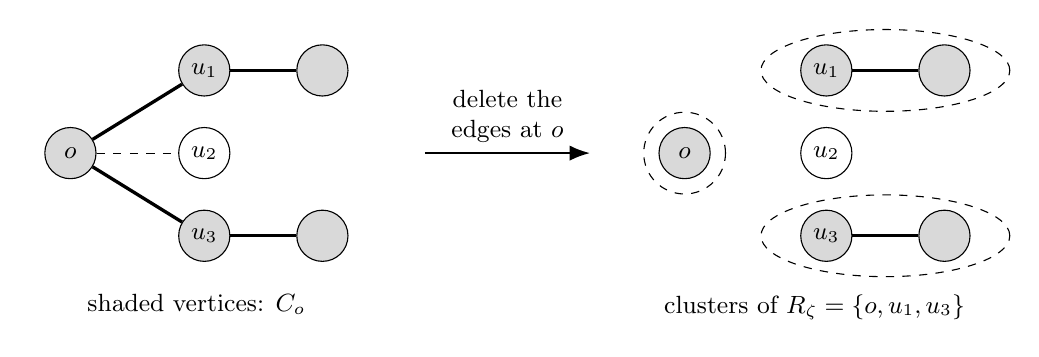
\begin{tikzpicture}[
  vtx/.style={circle,draw,fill=white,inner sep=0pt,minimum size=6.5mm,font=\small},
  inC/.style={vtx,fill=black!15},
  open/.style={line width=1.2pt}
]
  \node[inC] (o0)  at (0,0)      {$o$};
  \node[inC] (a0)  at (1.7,1.05) {$u_1$};
  \node[vtx] (b0)  at (1.7,0)    {$u_2$};
  \node[inC] (c0)  at (1.7,-1.05){$u_3$};
  \node[inC] (a0p) at (3.2,1.05) {};
  \node[inC] (c0p) at (3.2,-1.05){};
  \draw[open]   (o0)--(a0);
  \draw[dashed] (o0)--(b0);
  \draw[open]   (o0)--(c0);
  \draw[open]   (a0)--(a0p);
  \draw[open]   (c0)--(c0p);
  \node[fit=(o0)(a0)(c0)(a0p)(c0p),inner sep=6pt] (bx0) {};
  \node[anchor=north,font=\small] at (bx0.south) [yshift=-2pt] {shaded vertices: $C_o$};

  \draw[-{Latex[length=2.6mm]},thick] (4.5,0)--node[above,font=\small,align=center]
    {delete the\\edges at $o$}(6.6,0);

  \node[inC] (o1)  at (7.8,0)     {$o$};
  \node[inC] (a1)  at (9.6,1.05)  {$u_1$};
  \node[vtx] (b1)  at (9.6,0)     {$u_2$};
  \node[inC] (c1)  at (9.6,-1.05) {$u_3$};
  \node[inC] (a1p) at (11.1,1.05) {};
  \node[inC] (c1p) at (11.1,-1.05){};
  \draw[open] (a1)--(a1p);
  \draw[open] (c1)--(c1p);
  \begin{scope}[on background layer]
    \node[draw,dashed,ellipse,fit=(a1)(a1p),inner sep=1pt] {};
    \node[draw,dashed,ellipse,fit=(c1)(c1p),inner sep=1pt] {};
    \node[draw,dashed,circle,fit=(o1),inner sep=1pt] {};
  \end{scope}
  \node[fit=(o1)(a1)(c1)(a1p)(c1p),inner sep=6pt] (bx1) {};
  \node[anchor=north,font=\small] at (bx1.south) [yshift=-2pt]
    {clusters of $R_\zeta=\{o,u_1,u_3\}$};
\end{tikzpicture}
\caption{The state $\zeta$ of the edges at $o$ is fixed, and $R_\zeta$ collects $o$ together
with the endpoints of the open ones. In the graph with the edges at $o$ deleted, the union
of the clusters of the vertices of $R_\zeta$ equals the cluster $C_o$ of the original
configuration. The vertex $o$ is isolated there and contributes only itself, and the
remaining clusters need not be disjoint.}
\label{fig:star-exposure}
\end{figure}

\begin{theorem}\label{thm:q9}
Let $A$ be a nonempty finite set of vertices, let $o$ and $b$ be vertices, and let $a\in A$
satisfy $\PP_\star(a\con b)\leq\PP_\star(x\con b)$ for every $x\in A$. Then, with both
probabilities below evaluated under the original measure,
\[
 \PP(o\con b,o\con A)\geq\PP(o\con A,a\con b).
\]
\end{theorem}

\begin{proof}
Condition on the states of the edges incident to $o$. For an incident-edge configuration
$\zeta$, let
$R_\zeta$ be the union of $\{o\}$ and the set of vertices $u\neq o$ with $\{o,u\}$ open in
$\zeta$. The nonincident edges have exactly their law under $\PP_\star$, and they
are independent of $\zeta$.

Any open walk may be reduced to a simple path. Unless its endpoint is $o$, a simple path
from $o$ uses exactly one edge incident to $o$, as its first edge; the remaining path lies
in the graph with those incident edges deleted. Conversely, if
$u\in R_\zeta\setminus\{o\}$, every path in the deleted-edge graph beginning at $u$ can be
preceded by the open edge $\{o,u\}$; the isolated starting vertex $o$ contributes only
$o$. Hence, pointwise in the nonincident-edge configuration,
\begin{equation}\label{eq:star}
 C_o=C_{R_\zeta},\qquad \{o\con A\}=\{R_\zeta\con A\}\,,
\end{equation}
where $C_{R_\zeta}$ and $\{R_\zeta\con A\}$ are computed under $\PP_\star$, for which $o$ is isolated and therefore
contributes the single vertex $o$ to the union. Moreover, on $\{o\ncon a\}$ no path from
$a$ can use an edge incident to $o$. Hence $C_a$ in the original configuration equals the
cluster computed after deleting the incident edges.

Put $F=\one\{b\in\,\cdot\,\}$. On $\{o\con a\}$ the clusters of $o$ and $a$ coincide, so
\[
 \PP(o\con b,o\con A)-\PP(a\con b,o\con A)
 =\EE\bigl[F(C_o)-F(C_a);\ o\ncon a,\ o\con A\setminus\{a\}\bigr]\,,
\]
and by \eqref{eq:star} the right side equals
\[
 \sum_{\zeta}\PP\bigl(\text{the edges at $o$ have state }\zeta\bigr)\,
 \EE_\star\bigl[F(C_{R_\zeta})-F(C_a);\ R_\zeta\ncon a,\
 R_\zeta\con A\setminus\{a\}\bigr]\,,
\]
where the sum ranges over the states $\zeta$ of the edges at $o$,
the events and clusters inside the expectation being computed under $\PP_\star$. The
hypothesis on $a$ says $\EE_\star[F(C_a)]\leq\EE_\star[F(C_x)]$ for every $x\in A$, so each
summand is nonnegative by Theorem~\ref{thm:fm2} applied under $\PP_\star$ with the set
$R_\zeta$. Summing over $\zeta$ gives \eqref{eq:41}. No division is used, so states $\zeta$ of
probability zero and coincidences among $o$, $a$, $b$ and the vertices of $A$ are covered.
\end{proof}

The incident-edge decomposition does not apply to Question~8, whose minimizer is selected
on $\{o\ncon A\}$. We now give a counterexample to the proposed inequality.

\section{Question 8}\label{sec:q8}

Set
\[
 \rho_x=\PP(x\con b,\ o\ncon A)\qquad\text{for } x\in A\,.
\]
The phrase ``let $a$ minimize'' is understood to assert the conclusion for an
arbitrary minimizer. The choice matters when the minimum is attained more than once. The next
example lies on the boundary $\PP(o\ncon A)=0$: both vertices of $A$ minimize $\rho$, but
one of them violates \eqref{eq:41}. Thus Question~\ref{q8}, read as a statement about every
minimizer, is false. The example does not address an existential tie-breaking
interpretation.

\begin{proposition}\label{prop:q8}
There is a four-vertex weighted graph, a two-element set $A$, and vertices $o$ and $b$
outside $A$ with the following property. Both elements of $A$ minimize
$\PP(x\con b,\ o\ncon A)$, but one minimizing vertex $a$ satisfies
\[
 \PP(o\con b,\ o\con A)<\PP(o\con A,\ a\con b)\,.
\]
\end{proposition}

\begin{proof}
Let $V=\{o,a_1,a_2,b\}$ and $A=\{a_1,a_2\}$. Set
$p_{\{o,a_1\}}=p_{\{a_2,b\}}=1$, $p_{\{a_1,a_2\}}=\tfrac12$, and all other edge
probabilities to zero. Since $\{o,a_1\}$ is open with probability one and $a_1\in A$, the event $\{o\con A\}$
has probability one, so $\rho_{a_1}=\rho_{a_2}=0$ and both vertices minimize. The event
$\{a_2\con b\}$ has probability one, so $\PP(o\con A,\ a_2\con b)=1$. The event $\{o\con
b\}$ requires the edge $\{a_1,a_2\}$ to be open, so $\PP(o\con b,o\con A)=\tfrac12$. Thus
\eqref{eq:41} fails for $a=a_2$.
\end{proof}

The counterexample already has two intermediate vertices, so even the restriction
$|A|=2$ does not make \eqref{eq:41} valid. For completeness, we record two statements that
do hold when $|A|\leq2$: a unique minimizer works, and every minimizer works if
$\PP(o\ncon A)>0$. We first cancel the contribution from $\{o\con a\}$.

\begin{lemma}\label{lem:cancel}
Let $A$ be a nonempty finite set of vertices, let $a\in A$, and let $b$ and $o$ be
vertices. Then
\[
 \PP(o\con A,\ a\con b)-\PP(o\con b,\ o\con A)
 =\PP\bigl(a\con b,\ o\ncon a,\ o\con A\setminus\{a\}\bigr)
 -\PP\bigl(o\con b,\ o\ncon a,\ o\con A\setminus\{a\}\bigr)\,.
\]
\end{lemma}

\begin{proof}
Split $\{o\con A\}$ into $\{o\con a\}$ and $\{o\ncon a\}\cap\{o\con A\setminus\{a\}\}$. On
$\{o\con a\}$ the clusters of $o$ and $a$ coincide, so the events $\{a\con b\}$ and
$\{o\con b\}$ agree there and the two contributions from that part cancel.
\end{proof}

We use the following consequence of the BHK two-cluster inequality.

\begin{lemma}\label{lem:exch}
Let $S_1$ and $S_2$ be sets of vertices, let $g_3$ and $g_4$ be nonnegative real functions
of two edge sets, each increasing in the first argument and decreasing in the second, and
let $h_1$ and $h_2$ be nonnegative real functions of two edge sets, each decreasing in the
first argument and increasing in the second. Let $D=\{S_1\ncon S_2\}$ and define
$G_i(\omega)=g_i(\eC_{S_1}(\omega),\eC_{S_2}(\omega))$ and
$H_i(\omega)=h_i(\eC_{S_1}(\omega),\eC_{S_2}(\omega))$. Then
\[
 \EE[G_3H_1;D]\,\EE[G_4H_2;D]
 \leq \EE[G_3G_4;D]\,\EE[H_1H_2;D]\,.
\]
\end{lemma}

\begin{proof}
If $\PP(D)=0$, then both sides vanish, so assume $\PP(D)>0$.
Theorem~\ref{thm:bhk2} applies to $G_3,G_4$ and, after exchanging
$S_1$ and $S_2$, to $H_1,H_2$, giving
\[
 \EE[G_3;D]\,\EE[G_4;D]\leq\PP(D)\EE[G_3G_4;D],
 \quad
 \EE[H_1;D]\,\EE[H_2;D]\leq\PP(D)\EE[H_1H_2;D].
\]
Inequality~\eqref{eq:bhkneg} applies to $G_3,H_1$ and to $G_4,H_2$, giving
\[
 \PP(D)\EE[G_3H_1;D]\leq\EE[G_3;D]\EE[H_1;D],
 \quad
 \PP(D)\EE[G_4H_2;D]\leq\EE[G_4;D]\EE[H_2;D].
\]
All eight quantities are nonnegative. Multiplying the two inequalities of the second
display and then using the first display gives the asserted inequality after division by
$\PP(D)^2$.
\end{proof}

Lemma~\ref{lem:exch} controls the configurations that remain after the cancellation in
Lemma~\ref{lem:cancel}.

\begin{theorem}\label{thm:q8two}
Let $o$ and $b$ be vertices and let $A$ be a nonempty set of vertices with at most two
elements. If $a\in A$ is the unique vertex minimizing $\PP(x\con b,\ o\ncon A)$ over
$x\in A$, then
\[
 \PP(o\con b,\ o\con A)\geq\PP(o\con A,\ a\con b)\,.
\]
If $\PP(o\ncon A)>0$, then
\[
 \PP(o\con b,\ o\con A)\geq\PP(o\con A,\ a\con b)
\]
for every $a\in A$ that realizes the minimum.
\end{theorem}

\begin{proof}
We first treat $|A|=1$, then a strict minimum for $A=\{a,x\}$, and finally a tied minimum
under the assumption $\PP(o\ncon A)>0$.

If $A=\{a\}$, then on $\{o\con a\}$ the clusters of $o$ and $a$ coincide, so $\PP(o\con
A,a\con b)=\PP(o\con a,o\con b)=\PP(o\con b,o\con A)$, and both conclusions hold with
equality.

Next let $A=\{a,x\}$ with $\rho_a<\rho_x$. By Lemma~\ref{lem:cancel}, and because the
clusters of $o$ and $x$ coincide on $\{o\con x\}$, the inequality \eqref{eq:41} to be
proved reads
\begin{equation}\label{eq:q8target}
 \PP(a\con b,\ o\ncon a,\ o\con x)\leq \PP(x\con b,\ o\ncon a,\ o\con x)\,.
\end{equation}
Apply Lemma~\ref{lem:exch} with $S_1=\{a\}$ and $S_2=\{o,x\}$, and write $D$ for the event
$\{a\ncon o,\ a\ncon x\}$. For edge sets $K,L$, let $g_3(K,L)$ indicate that $a$ is
connected to $b$ using edges of $K$, and let $g_4(K,L)$ indicate that $o$ is not connected
to $x$ using edges of $L$. Let $h_1(K,L)$ and $h_2(K,L)$ indicate, respectively, that $o$ is
connected to $x$ using edges of $L$ and that $x$ is connected to $b$ using edges of $L$. Then $g_3,g_4$ are
increasing in $K$ and decreasing in $L$, while $h_1,h_2$ are decreasing in $K$ and
increasing in $L$. Evaluated at $(\eC_a,\eC_{\{o,x\}})$ on $D$, they are the four event
indicators just described.

On $\{o\con x\}$ the clusters of $o$ and $x$ coincide, so $a\ncon o$ is equivalent to
$a\ncon x$. Thus $D\cap\{o\con x\}=\{o\ncon a,\ o\con x\}$, and
\[
 \EE[g_3h_1;D]=\PP(a\con b,\ o\ncon a,\ o\con x),\qquad
 \EE[h_1h_2;D]=\PP(x\con b,\ o\ncon a,\ o\con x)\,.
\]
On the other hand $D\cap\{o\ncon x\}=\{o\ncon A\}\cap\{a\ncon x\}$. Two vertices connected
to $b$ are connected to each other. Thus, on $D\cap\{o\ncon x\}$, $\{a\con b\}$ implies $x\ncon b$, and
$\{x\con b\}$ implies $a\ncon b$. Therefore
\[
 \EE[g_3g_4;D]=\PP(o\ncon A,\ a\con b,\ x\ncon b),\qquad
 \EE[g_4h_2;D]=\PP(o\ncon A,\ x\con b,\ a\ncon b)\,,
\]
and Lemma~\ref{lem:exch} reads
\begin{equation}\label{eq:q8exch}
\begin{split}
 \PP(a\con b,\ o\ncon a,\ o\con x)\,&\PP(o\ncon A,\ x\con b,\ a\ncon b)\\
 &\leq \PP(o\ncon A,\ a\con b,\ x\ncon b)\,\PP(x\con b,\ o\ncon a,\ o\con x)\,.
\end{split}
\end{equation}
Splitting $\{o\ncon A,\ a\con b\}$ and $\{o\ncon A,\ x\con b\}$ according as the other
vertex of $A$ reaches $b$,
\begin{equation}\label{eq:q8-rho-split}
 \rho_a-\PP(o\ncon A,\ a\con b,\ x\ncon b)
 =\PP(o\ncon A,\ a\con b,\ x\con b)
 =\rho_x-\PP(o\ncon A,\ x\con b,\ a\ncon b)\,,
\end{equation}
Set
\[
 u=\PP(o\ncon A,a\con b,x\ncon b),\qquad
 v=\PP(o\ncon A,x\con b,a\ncon b).
\]
Equation~\eqref{eq:q8-rho-split} gives $v-u=\rho_x-\rho_a>0$, so $0\leq u<v$. If $L_a$ and $L_x$
denote the left- and right-hand probabilities in \eqref{eq:q8target}, then
\eqref{eq:q8exch} is $L_av\leq uL_x$. Hence
$L_a\leq(u/v)L_x\leq L_x$, proving \eqref{eq:q8target}.

The case $|A|=1$ and the strict two-vertex case prove the unique-minimizer clause.

For the positive-probability clause, assume $\PP(o\ncon A)>0$ and let $a$ realize the minimum. Again
only $A=\{a,x\}$ has to be treated, and only $\rho_a=\rho_x$.

Suppose first that $\rho_a=0$. A configuration has positive probability precisely when it
contains every edge of probability one and no edge of probability zero. Let $\omega_1$
contain exactly the probability-one edges. Choose a positive-probability configuration
$\eta\in\{o\ncon A\}$. Since $\omega_1\subseteq\eta$ and $\{o\ncon A\}$ is decreasing,
$\omega_1\in\{o\ncon A\}$.

Suppose $\PP(a\con b,o\ncon b)>0$. Choose a positive-probability configuration
$\xi\in\{a\con b,o\ncon b\}$ and a simple open path $\lambda$ from $a$ to $b$ in $\xi$. Write
$E(\lambda)$ for the set of edges of $\lambda$ and let $\omega=\omega_1\cup E(\lambda)$. This configuration has positive probability,
$\omega\subseteq\xi$, and $a\con b$ in $\omega$. Moreover $o\ncon A$ in $\omega$. Indeed,
a path from $o$ to $A$ that uses only edges of $\omega_1$ would contradict
$\omega_1\in\{o\ncon A\}$. Every other such path uses an edge of $E(\lambda)$ and would therefore connect $o$ to $b$ in
$\omega$, hence in $\xi$, contradicting the choice of $\xi$. Thus $\rho_a>0$, a
contradiction. Hence $\{a\con b\}$ is contained in $\{o\con b\}$ up to a null event. On
$\{a\con b\}\cap\{o\con b\}$, the vertices $o$ and $a$ are connected through $b$, so
$\{o\con A\}$ holds as well; therefore $\PP(o\con A,a\con b)\leq\PP(a\con b)\leq\PP(o\con
b,o\con A)$.

Suppose finally that $\rho_a>0$, and fix $q$ with $0<q<1$. Enlarge the vertex set by one
vertex $y$, set $p_{\{y,a\}}=q$ and all other edge probabilities incident to $y$ to zero,
leave every old probability unchanged, and replace $A$ by $\{y,x\}$; write $\PP_q$ for the
enlarged measure. Condition on the state of $\{y,a\}$. If the edge $\{y,a\}$ is open, then $y$ is
joined exactly to the vertices of the cluster of $a$, the connections among the old
vertices are unchanged, and the events $\{o\con\{y,x\}\}$ and $\{y\con b\}$ are $\{o\con
A\}$ and $\{a\con b\}$. If the edge $\{y,a\}$ is closed, then $y$ is isolated, so $\{y\con b\}$ is empty
and $\{o\con\{y,x\}\}$ is $\{o\con x\}$. Hence
\[
 \PP_q(y\con b,\ o\ncon\{y,x\})=q\rho_a,\qquad
 \PP_q(x\con b,\ o\ncon\{y,x\})=q\rho_x+(1-q)\PP(x\con b,\ o\ncon x)\,,
\]
\[
 \PP_q(o\con\{y,x\},\ y\con b)=q\,\PP(o\con A,\ a\con b)\,,
\]
\[
 \PP_q(o\con b,\ o\con\{y,x\})=q\,\PP(o\con b,\ o\con A)+(1-q)\,\PP(o\con b,\ o\con x)\,.
\]
Let

be the two quantities minimized in the enlarged graph. Since
$\{o\ncon A\}\subseteq\{o\ncon x\}$, we have
$q\rho_x+(1-q)\PP(x\con b,o\ncon x)\geq\rho_x=\rho_a>q\rho_a$. Thus $y$ is the unique
minimizer in $\{y,x\}$.
The unique-minimizer case just proved gives
\begin{equation}\label{eq:q8-unique-applied}
 q\,\PP(o\con A,\ a\con b)\leq q\,\PP(o\con b,\ o\con A)+(1-q)\,\PP(o\con b,\ o\con x)\,.
\end{equation}
Suppose $\delta=\PP(o\con A,a\con b)-\PP(o\con b,o\con A)$ is positive; then $\delta\leq1$,
and \eqref{eq:q8-unique-applied} gives
$q\delta\leq(1-q)\PP(o\con b,o\con x)\leq1-q$ for every $q$ with $0<q<1$. Taking
$q=1-\delta/4\in[3/4,1)$ turns this into
$(1-\delta/4)\delta\leq\delta/4$, that is $\delta\geq3$, a contradiction. Hence $\delta\leq0$,
which is \eqref{eq:41}.
\end{proof}

\begin{remark}
The present argument does not determine whether \eqref{eq:41} holds for the unique minimizer of $\rho_x$ when
$|A|\geq3$. By contrast, if $a$ minimizes $\PP(o\con A,x\con b)$ over $x\in A$, then
\eqref{eq:pre} gives \eqref{eq:41}.
\end{remark}

We conclude by specifying the scope of the accompanying Lean verification.

\section{Lean Verification}\label{sec:lean}

The accompanying Lean formalization checks Conjectures~\ref{c1}--\ref{c4} and~\ref{c6},
Questions~\ref{q5}, \ref{q7}, and~\ref{q9}, and the counterexample in
Proposition~\ref{prop:q8}. It also checks the strong pre-FKG inequality, the form of
Conjecture~\ref{c4} with the minimizing vertex prescribed, the stronger form of Conjecture~\ref{c6}, and
Theorem~\ref{thm:fm2}. These declarations build on the Lean proof of
Theorem~\ref{thm:csh}, named \texttt{Percolation.Continuity.CSH.cshHolds}, in \cite{Dev}.
Three of the correspondences are not literal. The declaration \texttt{KNAll.genY\_all}
yields Theorem~\ref{thm:gen} after the finite real-valued order on $T$ is replaced by an
order-equivalent rank with values in the natural numbers, extended arbitrarily off $T$. The
declaration \texttt{KNAll.setSourceFixedMin\_holds} proves Theorem~\ref{thm:fm2} and also
covers the empty source. The formal Conjecture~\ref{c3} quantifies over the empty set $A$ as
well, and the formal Conjecture~\ref{c6} also covers the degenerate pair $v=w$, whereas the
statements above take $A$ nonempty and the two endpoints of $e$ distinct.

The cluster-exploration inputs in Section~\ref{sec:inputs} are also machine-checked. The
conditional-mean identity is
\nolinkurl{Percolation.Continuity.CSH.residual_orthogonal}; the positivity and
monotonicity of $\Psi$ are \nolinkurl{Percolation.Continuity.CSH.phiFun_nonneg} and
\nolinkurl{Percolation.Continuity.CSH.phiFun_mono}; and \eqref{eq:markov1} is the form for a set of
vertices \nolinkurl{KNAll.Guarded.guardResid_sourceCluster}. The stopped estimate
\eqref{eq:stopped} and its monotonicity use
\nolinkurl{Percolation.Continuity.CovTauStarN.yS_mul_mS_le} and
\nolinkurl{Percolation.Continuity.CovTau.Yw_antitone_of_le}. Their set-source specialization is checked in
\nolinkurl{KN/GuardedKernel.lean} as part of the public declaration
\nolinkurl{KNAll.Guarded.guardHorizontal_nonneg}.

Two results in this paper are not part of the current Lean certificate. The formal
theorem for Question~\ref{q5} has the right side $\PP(o\con b)$ printed by Kozma and Nitzan;
the sharper right side $\PP(o\con b,\ o\con A)$ in Theorem~\ref{thm:q5} is proved here.
The positive two-vertex result in Theorem~\ref{thm:q8two} is also proved only in this
paper.

\begingroup
\raggedright
\hbadness=10000
\setlength{\parindent}{1.5em}
\setlength{\emergencystretch}{4em}
The principal declarations are \texttt{KNAll.genY\_all} for Theorem~\ref{thm:gen},
\texttt{KNAll.conjecture4Fixed\_holds} for Theorem~\ref{thm:fixedmin}, and
\texttt{KNAll.setSourceFixedMin\_holds} for Theorem~\ref{thm:fm2}. The declarations
\texttt{KNAll.conjecture1\_holds}, \texttt{KNAll.conjecture2\_holds},
\texttt{KNAll.conjecture2Strong\_holds}, \texttt{KNAll.conjecture3\_holds},
\texttt{KNAll.conjecture4\_holds},
\texttt{KNAll.conjecture4\_clusterProperty\_holds}, and
\texttt{KNAll.question7\_holds} cover the consequences in
Section~\ref{sec:proj}. Question~\ref{q5} is \texttt{KNAll.question5\_holds}.
Conjecture~\ref{c6} and its strengthening are \texttt{KNAll.Guarded.conjecture6\_holds}
and \texttt{KNAll.Guarded.conjecture6Strong\_holds}. Question~\ref{q9} is
\texttt{KNAll.question9\_holds}, obtained by combining
\texttt{KNAll.setSourceFixedMin\_holds} with
\texttt{KNAll.question9\_of\_setSourceFixedMin}. The counterexample to
Question~\ref{q8} is \texttt{KNAll.not\_question8EveryMin}.

Each listed declaration compiles under Lean \texttt{4.32.0} with no \texttt{sorry} and
depends only on the axioms \texttt{propext}, \texttt{Classical.choice}, and
\texttt{Quot.sound}. The Mathlib commit is
\[
 \texttt{81a5d257c8e410db227a6665ed08f64fea08e997}.
\]
\endgroup

\begin{thebibliography}{BHK06}
\setlength{\itemsep}{1pt}\setlength{\parskip}{0pt}

\bibitem[AD78]{AD} R.~Ahlswede and D.~E.~Daykin, \emph{An inequality for the weights of two
families of sets, their unions and intersections}, Z.~Wahrscheinlichkeitstheorie verw.\
Gebiete \textbf{43} (1978), 183--185.

\bibitem[BHK06]{BHK} J.~van den Berg, O.~H\"aggstr\"om and J.~Kahn, \emph{Some conditional
correlation inequalities for percolation and related processes}, Random Structures
Algorithms \textbf{29} (2006), 417--435. Theorem 1.1 (p.~3) gives
Theorem~\ref{thm:bhk}. At $q=1$, Theorem 2.1 (p.~9) follows from Theorem 1.5 (p.~7) and
Remark 1 (p.~5); these give Theorem~\ref{thm:bhk2}.

\bibitem[Dev26]{Dev} \emph{Theta at the critical point vanishes for Bernoulli bond
percolation on the hypercubic lattice in all dimensions at least two, in Lean 4 and
Mathlib}, 2026, \url{https://github.com/anthropics/formal-math/tree/795efb86f191735c5481675763537cfb4ff37e55/percolation}.

\bibitem[Gla24]{Gladkov24} N.~Gladkov, \emph{Percolation inequalities and decision trees},
arXiv:2408.08457v2, 2024.

\bibitem[H60]{H} T.~E.~Harris, \emph{A lower bound for the critical probability in a certain
percolation process}, Proc.\ Cambridge Philos.\ Soc.\ \textbf{56} (1960), 13--20.

\bibitem[KN24]{KN} G.~Kozma and S.~Nitzan, \emph{A reduction of the percolation at
criticality problem to a conjectured inequality}, arXiv:2401.12397, 2024. Conjectures~1--3
with display (3) are on pp.~3 and~15, Conjecture~4 and Question~5 on pp.~31--32,
Conjecture~6 on p.~34, and Questions~7--9 with display (41) on p.~36.

\end{thebibliography}

\end{document}
